\section{Post-Training}
\label{sec:posttraining}

Given the pretrained model, we conduct a post-training phase that has been substantially redesigned from the pipeline used for Nemotron 3 Super~\citep{nvidia2026nemotron3superopen}. As illustrated in Figure~\ref{fig:posttraining_stages}, the pipeline starts with a general Supervised Fine-tuning stage. Instead of relying solely on consecutive reinforcement learning stages, we augment the pipeline with Multi-teacher On-Policy Distillation (MOPD)~\citep{yang2026nemotron,lu2025onpolicydistillation,xiao2026mimo}, enabling both broad capability acquisition and targeted specialization. The remainder of this section is organized around the MOPD process: we first describe how the student model is prepared through SFT, RLVR, and MOPD warmup, then present the training of specialized teacher models, and finally detail the iterative MOPD optimization and MTP Boosting procedures.


\begin{figure}[h]
    \centering
    % \includegraphics[width=0.9\linewidth]{figures/posttrain-pipeline.pdf}
    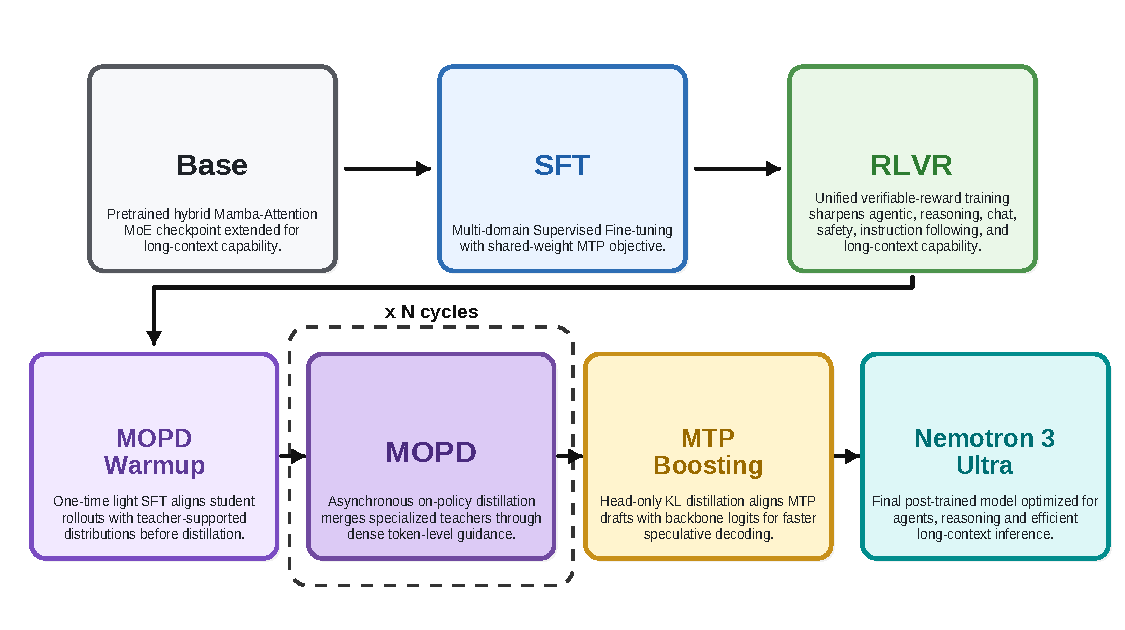
\includegraphics[width=0.9\linewidth]{figures/nemotron3_ultra_pipeline_two_row_larger_text.pdf}
    \vspace{-0.5em}
    \caption{Overview of the post-training pipeline for \ourmodel.}
    \label{fig:posttraining_stages}
    \vspace{-0.5em}
\end{figure}


\subsection{Supervised Fine Tuning}
\label{subsec:SFT}

% \todo{Wenliang: New data that was added for SFT. Other SFT details}

% To train the student model, starting from the pre-trained base model, we first conduct Supervised Fine Tuning (SFT) using packed sequences of length $294{,}912$ with a batch size of 64. We train for $166{,}400$ samples using a cosine learning-rate scheduler with peak learning rate $1.5e\!-\!5$ and minimum learning rate $1e\!-\!6$, and 9{,}600 warmup samples. As in pre-training, we retain the shared-weight MTP objective during SFT, using two MTP layers with per-token auxiliary loss scaling factor 0.1. 

% To train the student model, we start from the pre-trained base model and perform Supervised Fine-Tuning (SFT) on packed sequences of length $294{,}912$ with a global batch size of $64$. We train on $204{,}800$ samples using a cosine learning-rate schedule with a peak learning rate of $1.5 \times 10^{-5}$, a minimum learning rate of $1 \times 10^{-6}$, and $9{,}600$ warmup samples. 

% % We optimize a sequence-averaged token-level cross-entropy loss. Let the global batch consist of $B$ packed sequences, where sequence $i$ contains $T_i$ supervised (response) tokens with per-token loss $\ell_{i,t}$; prompt tokens are masked out. We first average the loss over the supervised tokens within each sequence, then average uniformly across the $B$ sequences in the batch:
% % \begin{equation*}
% % \mathcal{L} = \frac{1}{B} \sum_{i=1}^{B} \frac{1}{T_i} \sum_{t=1}^{T_i} \ell_{i,t},
% % \end{equation*}
% % Since packs are filled to a nearly constant total length but only response tokens are supervised, this normalization prevents response-dense packs (e.g., short-prompt/long-response data) from dominating the update, yielding a more balanced objective across heterogeneous input/output length ratios.

% As in pre-training, we retain the shared-weight MTP objective during SFT, using two MTP layers with a per-token auxiliary-loss scaling factor of $0.1$. 

To train the student model, we start from the pre-trained base model and perform Supervised Fine-Tuning (SFT) in two stages, following \supermodel~\citep{nvidia2026nemotron3superopen}. In Stage~1, we train on packed sequences of length $294{,}912$ tokens with global batch size $64$ for $204{,}800$ samples, using a cosine learning-rate schedule with peak learning rate $1.5 \times 10^{-5}$, minimum learning rate $1 \times 10^{-6}$, and $9{,}600$ warmup samples. In Stage~2, we extend packed sequence to $515{,}000$ tokens, augmenting the mixture with additional long-context data up to $512$K tokens. We train with global batch size $64$ for $19{,}200$ samples, using the same learning-rate schedule with peak $1 \times 10^{-5}$ to minimum $2 \times 10^{-6}$ and $6{,}400$ warmup samples. 
% Since long-context examples typically contain many prompt/context tokens but relatively few supervised output tokens, Stage~2 uses per-sequence normalization to prevent response-dense shorter examples from dominating the update. This combination of longer packed-sequence training and sample-level normalization better balances short-context reasoning with long-context capability. 
As in pre-training, we retain the shared-weight MTP objective during SFT, using two MTP layers with a per-token auxiliary-loss scaling factor of $0.1$.

\subsubsection{Data}
\paragraph{Long Context.}
We prepare 512K long-context SFT data based on the synthetic data pipeline following~\citep{nvidia2026nemotron3superopen}. 
Our data is aimed at improving long-context abilities including, but not limited to multi-document reasoning, sequential scanning, and querying synthetic tables.
%Our data is aimed at improving the abilities including long-context multi-document reasoning, sequential scanning, and SQL queries. 
\paragraph{Efficiency and Control.}
The SFT data include two components for reasoning efficiency and control. The first is training samples
generated by GPT-OSS-120B in its medium-effort mode on prompts of math reasoning, STEM question answering and instruction following. These SFT data initiate Ultra's medium-effort mode which is later optimized during the RLVR stage. The second component is training samples where the reasoning traces are truncated to random reasoning budgets while the responses remain the same. This is similar to Nemotron 3 Nano and Super with one design change: the \texttt{</think>} tokens in the truncated samples are masked from SFT training loss.


\paragraph{Safety.}
To instill robust safety behaviors, first, we retain the $45$K safety data blend curated in \supermodel~\citep{nvidia2026nemotron3superopen} with prompts curated from diverse sources and responses synthetically generated conditioned on a response policy mapped to each prompt. Our two-stage response and reasoning generation framework enables deliberate reflection on safety guidelines in the reasoning traces and ensures that the final responses are consistent, policy-compliant, and contextually appropriate. Further, to curate a multilingual set for \ourmodel training, we translated the \supermodel safety data blend into six languages — German, Spanish, French, Japanese, Italian, and Chinese - using NeMo Skills' chunked translation capability, ensuring sentence-by-sentence parity, and paired with NVIDIA Riva Translate 4B v1.1 as the translation backbone. 

To improve translation quality, each translated example was back-translated into English and compared against the original English prompt-response pair. Examples with semantic similarity below 0.8 were filtered out, removing approximately $\approx10 - 15\%$ of examples per translated language. The highest- and lowest-scoring translations were manually spot-checked to verify that this filter was removing examples with clear translation failures or structural issues. After filtering, we used stratified sampling to create a balanced dataset across the six translated languages. The final safety blend contains about $\approx135$K samples: $\approx45$K in English and $\approx15$K from each of the translated languages.
% in \texttt{de}, \texttt{es}, \texttt{fr}, \texttt{ja}, \texttt{it}, and \texttt{zh}.

\paragraph{Search Capabilities.}
During SFT, we expose the model to search data spanning different difficulty levels and tool-use harnesses to improve generalization.

First, we retain the search trajectories from the \supermodel~\citep{nvidia2026nemotron3superopen} dataset, whose seed prompts are grounded in the Wikidata knowledge graph. Specifically, the dataset selects well-connected hub entities and performs 4--8 hop random walks over factual relations to construct multi-hop search prompts. These prompts are then solved using Tavily Search Engine (\url{https://www.tavily.com/}), with MiniMax 2.1 serving as the teacher model.

In addition, we include a new search dataset: a commercially cleared subset of OpenResearcher~\citep{li2026openresearcher}, a public SFT dataset designed for long-horizon research agents. OpenResearcher synthesizes over $97$K trajectories using \texttt{gpt-oss-120b}~\citep{agarwal2025gpt} as the teacher model in a fully offline browser environment. The environment is backed by a local search index over $15$M FineWeb documents~\citep{penedo2024fineweb} augmented with bootstrapped evidence documents, and exposes three structured browser tools: \texttt{search} for retrieving candidate pages, \texttt{open} for inspecting full document contents, and \texttt{find} for locating exact textual evidence within an opened document. The resulting trajectories capture long-horizon reasoning-action-observation loops in which the model iteratively decomposes research questions, gathers and inspects sources, localizes supporting evidence, and synthesizes grounded final answers. For \ourmodel, we did not regenerate the OpenResearcher data; instead, we curated the commercial-OK portion by removing examples whose source licensing was not cleared for commercial use. This filtering yields approximately $21.7$K SFT trajectories while preserving the original browser-tool interaction format for training open-ended research and evidence-grounded search behavior.

Finally, we work with data vendors to curate particularly challenging samples that require 50--100 searches, and collect SFT trajectories in our BrowseComp harness, described in Appendix~\ref{appendix:eval}. For these trajectories, we use MiniMax 2.5 and GLM 5.1 as teacher models.


\paragraph{Terminal-Use Capabilities.}
% \todo{Khushi / Charlie / Venkat}
To develop strong terminal-use capabilities, we constructed a large-scale dataset of synthetic agentic trajectories covering a broad range of terminal tasks, including software engineering, data processing, file operations, and scientific computing. Seed instructions were sourced from a combination of publicly available datasets: OpenCodeReasoning \citep{nvidia2025opencodeReasoning}, OpenMathReasoning \citep{nvidia2025openmathReasoning}, SWE-bench \citep{jimenez2024swebenchlanguagemodelsresolve}, SWE-Fixer-Train-110K \citep{swefixer2025}, SWE-rebench \citep{badertdinov2025swerebenchautomatedpipelinetask}, and SWE-smith \citep{pan2025swesmith}. Tasks were assembled from two complementary sources: one portion was adapted from existing math and coding SFT data in Nemotron-Cascade, reformatted to align with the terminal-use environment, while the other was synthetically generated using DeepSeek-V3.2 \citep{deepseekai2025deepseekv3technicalreport} to cover a wider variety of terminal scenarios not well-represented in existing benchmarks. For trajectory generation, DeepSeek-V3.2 was used as the acting agent within the Terminus-2 agent provided by the Harbor framework \citep{harbor2025}. Each trajectory unfolds over multiple episodes in which the model receives an initial task prompt and subsequently interacts with a live terminal environment, issuing commands and incorporating execution feedback to make iterative progress toward task completion. This multi-step, environment-grounded collection process encourages the model to learn practical tool use, adaptive planning, and error recovery behaviors that are characteristic of effective terminal operation. The final dataset comprises approximately 370K multi-turn conversations, consisting of a mixture of reasoning and non-reasoning trajectories.

\paragraph{Conversational Tool Use Capabilities.}
We scale conversational tool-use data via a fully
synthetic, six-stage generation pipeline. This includes User and Environment simulation. This pipeline is similar to what is described in Nemotron-3 Super. 

\paragraph{Software Issue Resolution.}
% \todo{@Sugam / Som / Wasi - SWE data}
To distill robust problem solving capabilities, we curated a diverse dataset of synthetic agent trajectories focused on resolving real-world GitHub issues. To this end, we generated synthetic trajectories by leveraging two distinct modeling paradigms: the reasoning-based (thinking) Minimax-M2.5 \citep{minimax2026m25} and the instruction-based (non-thinking) Qwen3-Coder-480B-A35B-Instruct \citep{yang2025qwen3technicalreport} for issue resolution. The underlying issue statements were curated from a diverse set of publicly available datasets, including SWE-Gym \citep{pan2025trainingsoftwareengineeringagents}, R2E-Gym \citep{jain2025r2egymproceduralenvironmentshybrid}, SWE-rebench \citep{badertdinov2025swerebenchautomatedpipelinetask}, and SWE-rebench-V2 \citep{badertdinov2026swe}. These trajectories were captured using the OpenHands \citep{wang2025openhandsopenplatformai}, SWE-agent \citep{yang2024sweagent}, and Mini-SWE-agent and Opencode harnesses. Raw agent rollouts contain many patterns that, while completing the task, would teach undesirable behaviors if used directly as SFT data, so we filter the rollout pool with a per-trajectory heuristic analyzer evaluates a fixed set of signals to make an include/exclude decision: submission
  integrity (trajectory must end with a valid submission action), disallowed git operations (any use of push, pull, fetch, clone, cherry-pick, reflog, fsck, remote, or ls-remote), edit-test loop anti-patterns (the model thrashes between edits and test runs without converging — either reverting its own edits or repeating the edit → test → edit cycle indefinitely), lost-in-exploration (the model spends most of its turns reading/searching the repo but rarely edits, indicating failure to localize and commit to a fix), tool-call hygiene (high rate of malformed tool calls), debug-artifact detection in the final patch (print(, pdb, breakpoint()), and a verification check that flags trajectories that edit but never run tests. This multi-model, multi-framework approach ensures the resulting dataset promotes generalization across both diverse problem-solving modes and varied agentic environments. 

\paragraph{Math / Proof Data.}
We use the Nemotron-Cascade-2~\citep{yang2026nemotron} math data, which sources problems primarily from Nemotron-Cascade~\citep{wang2025nemotroncascadescalingcascadedreinforcement,liu2025acereason} and Nemotron-Math-V2~\citep{du2025nemotronmath}.
For the non-proof math data, we collect 1.8M tool-calling samples and 1.9M non-tool samples, with responses generated by DeepSeek-V3.2 and DeepSeek-V3.2-Speciale, respectively.
For the mathematical natural language proof data, we source proof problems from the AOPS split of Nemotron-Math-Proofs-v1~\citep{du2025nemotronmath} and generate responses from DeepSeek-V3.2-Speciale for capabilities including proof generation, proof verification, and proof refinement.

\paragraph{Science.}
We prepare our science SFT data following the Nemotron Nano recipe~\citep{nvidia2025nemotron3nanoopen}, which combines synthetic, real-world, and document-derived seed data spanning physics, chemistry, and biology. Prompts and formats are diversified using NeMo Data Designer~\citep{nemo-data-designer}, and the resulting samples are filtered with an LLM judge for format compliance and reasoning quality. In addition to the Nano recipe, we generate web-search and web-search-with-Python reasoning traces using DeepSeek-V3.2~\citep{deepseekai2024deepseekv32}. For web-search traces, the model is provided access to the Tavily search engine (\url{https://www.tavily.com/}); for web-search-with-Python traces, the model additionally has access to a Python execution environment.

\paragraph{Chat.}
We create multi-turn chat SFT data by starting from seed prompts drawn from open conversational datasets such as LMArena \citep{chiang2024chatbot} and WildChat \citep{li2024wildchat}. For each prompt, we sample multiple candidate responses from GLM-5 \citep{glm5team2026glm5vibecodingagentic} and use Nemotron-GenRM \citep{Wang2025HelpSteer3Preference} to select the highest-quality response for the current turn. To extend the data into multi-turn conversations, we simulate the user with the same LLM under controlled prompting. The simulated user is guided by hand-crafted conversation strategies, such as building on prior content, asking for clarification, challenging assumptions, reframing the task, or applying the answer to a new context, in order to produce diverse and realistic dialogue trajectories. To build multi-turn robustness, we construct examples in which earlier assistant turns may contain suboptimal responses rather than the best-ranked candidates. The model is trained only on the final assistant response in SFT to produce high-quality current-turn outputs while remaining robust to imperfect previous turns.

\paragraph{Code.}
We collect our coding problems from modern competitive programming platforms such as Codeforces, AtCoder, AIZU, and CodeChef. Following \citet{yang2026nemotron}, we applied strict deduplication and aggressive filtering to improve the data quality and balance the problem difficulties. We choose GPT-OSS-120B~\citep{agarwal2025gpt} as our teacher model with the consideration of their strong reasoning ability and good verbosity, and apply the rejection sampling on those reasoning traces. This pipeline yields a final dataset comprising 1.2M Python reasoning traces, 1.0M C++14 reasoning traces, and 1.3M Python tool-calling reasoning traces for competitive coding.

\paragraph{CUDA.}
%@Jingquan Wang US - Cuda data
We constructed a large-scale synthetic CUDA dataset comprising approximately 100K samples for kernel generation, repair, and optimization. The dataset was built using an LLM-based synthetic data generation pipeline with DeepSeek-R1 and GPT-OSS-120B. Seed questions were sourced from popular open-source libraries, NVIDIA library API surfaces, and BackendBench~\citep{saroufimbackendbench}. The construction was motivated by the need for CUDA-specialized training data that reflects real-world GPU-kernel programming and benchmarking challenges, as highlighted by recent CUDA benchmark efforts such as SOL-ExecBench~\citep{lin2026solexecbenchspeedoflightbenchmarkingrealworld}. These seeds were used to generate two types of samples: \emph{PyTorch-reference-to-CUDA-kernel} samples and \emph{natural-language-specification-to-CUDA-kernel} samples, with each sample accompanied by reasoning. For each seed item, multiple candidate kernels were produced through LLM-based synthetic generation and rejection sampling. Candidate kernels were validated in an internal CUDA evaluation environment using compilation checks, numerical correctness tests, and runtime benchmarking. Invalid, non-compiling, or incorrect candidates were rejected. Among the remaining valid candidates, the best-performing kernel according to benchmarked runtime was retained. In addition, we collected traces from an internal CUDA agent to produce repair and optimization data. The repair samples contain a PyTorch reference, a faulty CUDA C++ kernel, the corresponding error message, and a corrected CUDA C++ kernel. The optimization samples contain a PyTorch reference, a slow CUDA C++ kernel, an Nsight Compute log, and an optimized CUDA C++ kernel. Beyond direct CUDA C++ kernel generation, we also generated CUDA-X library  data using publicly available documentation and official code samples. Following the same formulation as the CUDA-C data, we generated PyTorch references, aligned natural-language specifications, corresponding CUDA-X library implementations, and reasoning. The covered libraries include Thrust, CUB, cuBLAS, cuDNN, cuSPARSE, cuRAND, and cuSOLVER.

\paragraph{RTL.}
%@Chenhui Deng US RTL data
We use the ACE-RTL~\citep{deng2026ace} training data, which covers three major RTL task categories: specification-to-RTL generation, code editing, and code debugging. ACE-RTL builds on the seed RTL corpus from ScaleRTL~\citep{deng2025scalertl}, where seed designs are collected from license-checked open-source RTL repositories and processed through deduplication, filtering, and syntax validation before being used for data generation. For specification-to-RTL tasks, DeepSeek-R1 and GPT-OSS-120B are used to synthesize natural-language specifications paired with the corresponding golden RTL implementations derived from the seed designs. For editing and debugging tasks, the original seed RTL is treated as the golden implementation, while simplified variants with missing functionality or buggy variants with realistic injected design errors are generated as inputs; the corresponding specifications describe either the required feature extensions or diagnostic information needed to recover the golden RTL. After further filtering through syntax checks, benchmark decontamination, and semantic-alignment evaluation using human-defined rubrics, the final dataset contains around 1.2M training samples.

\paragraph{Multilingual.}
Our multilingual post-training data is a mixture of sentence-level parallel corpora and synthetic translations of English SFT examples in math, code, and science domains.
For the synthetic data, driven by data quality issues identified in the previous line-by-line translation pipeline, we introduced a new end-to-end translation pipeline that takes the full JSON object as input and generates the full JSON object as output.
Because this pipeline requires strong long-context capabilities from the translation model, we transitioned to \texttt{DeepSeek-V3-0324}.
After translation, we first perform heuristic format checking to ensure all outputs conform to the specified JSON format, followed by the same data filtration steps and light-weight post-editing step introduced in the Nemotron Super-V3 recipe~\citep{nvidia2026nemotron3superopen}.
Ablation studies on Japanese data showed significant improvements measured by MMLU-ProX~\citep{xuan2025mmluprox}, confirming quality improvements over the line-by-line pipeline.
For Nemotron Ultra-V3, we synthesized data for Hindi, Japanese, Korean, and Brazilian Portuguese using this pipeline, while reusing existing multilingual synthetic data from Super-V3 for the remaining languages.

\subsubsection{Data Packing}
% @Wenliang - Blending / packing details
To train efficiently on a large and diverse collection of datasets, we adopt a length-aware best-fit packing strategy~\citep{ding2024fewer}, which packs multiple conversations into sequences up to a maximum context length. 
Our packer is highly memory-efficient: it reads and interleaves all source files in a round-robin fashion, maintains only a fixed-size pool of open sequences in memory, and retires a sequence once its residual capacity falls below a small tolerance. 
Each incoming conversation is assigned to the partially filled sequence whose remaining capacity it most tightly fits, following a best-fit rule that minimizes padding overhead. 
We neither truncate nor split conversations, preserving complete context and reducing hallucinations. 
Additionally, we enforce an in-pack deduplication constraint to prevent identical prompts from co-occurring within the same sequence. 
After packing, we perform a final shuffle over all completed packs. 
Overall, our implementation ensures that each packed sequence draws from a broad, well-mixed cross-section of the data distribution rather than clustering examples from any single source. 
This thorough mixing is essential at scale, where naive concatenation of per-source shards would otherwise induce strong distributional locality and degrade optimization stability.
\subsection{Reinforcement Learning}
\label{subsec:RL}



To improve upon SFT model, we conduct a unified RLVR (Reinforcement Learning with Verifiable Reward) training stage spanning all available environments, targeting terminal usage, office and productivity workflows, software engineering, search, general tool-calling, math, code, STEM, safety, chat, instruction following, long-context QA, inductive and transductive reasoning, structured outputs, and general model usability. For harness-based environments, we construct training data using a diverse collection of harness implementations and interaction formats, improving robustness to variations in execution settings and reducing overfitting to any particular harness design.

We refresh the RL training data using recent collections and perform reward profiling prior to training. For data mixture and curriculum construction, we adopt the Gaussian-based approach introduced in~\cite{nvidia2025nemotron3nanoopen}. Our training procedure largely follows the asynchronous GRPO algorithm with the stability optimizations proposed in~\cite{nvidia2026nemotron3superopen}, while incorporating several improvements to the training infrastructure, detailed in Section~\ref{subsec:infrastructure}. To support training across a large and diverse set of environments, we use a global batch size of 8192, with each sample generating 16 rollouts. Training begins with a maximum generation length of 48K tokens, which is later increased to 64K tokens. % Unlinking Appendix from here until we actually write something there % Please refer to Appendix \ref{appendix:rlvr} for some targeted upgrades to our RLVR environments compared to \supermodel.
% \todo{folks to add new RLVR envs as appendix sections, if they'd like.}
\subsection{MOPD}
\label{subsec:MOPD}

Mixed-environment RLVR provides broad capability improvements across a wide range of domains. However, as the number of environments continues to grow, each domain contributes only a relatively small number of samples to any given training batch, diluting the per-domain learning signal and making it increasingly difficult to balance training across domains. To fully unlock performance and push the frontier in each capability area, we train more than ten specialized teacher models, each optimized through its own domain-specific training pipeline.

During MOPD, the student model (obtained from RLVR) generates rollouts across all domains and receives dense reward signals from the corresponding teacher models. To maximize efficiency, MOPD is conducted asynchronously, with student rollout generation, teacher scoring, and student optimization fully pipelined. Moreover, MOPD is performed over multiple iterative cycles: after obtaining an MOPD-trained checkpoint, we branch out new rounds of teacher training initialized from the updated student model and subsequently merge the resulting improvements back into the next MOPD stage. This iterative co-evolution between student and teachers enables continuous capability improvement and progressively stronger specialization across domains. On training Nemotron 3 Ultra, we conduct two iterations of MOPD, with exact procedure shown in Figure~\ref{fig:mopd_detail}.



\begin{figure}[h]
    \centering
    % \includegraphics[width=0.9\linewidth]{figures/posttrain-pipeline.pdf}
    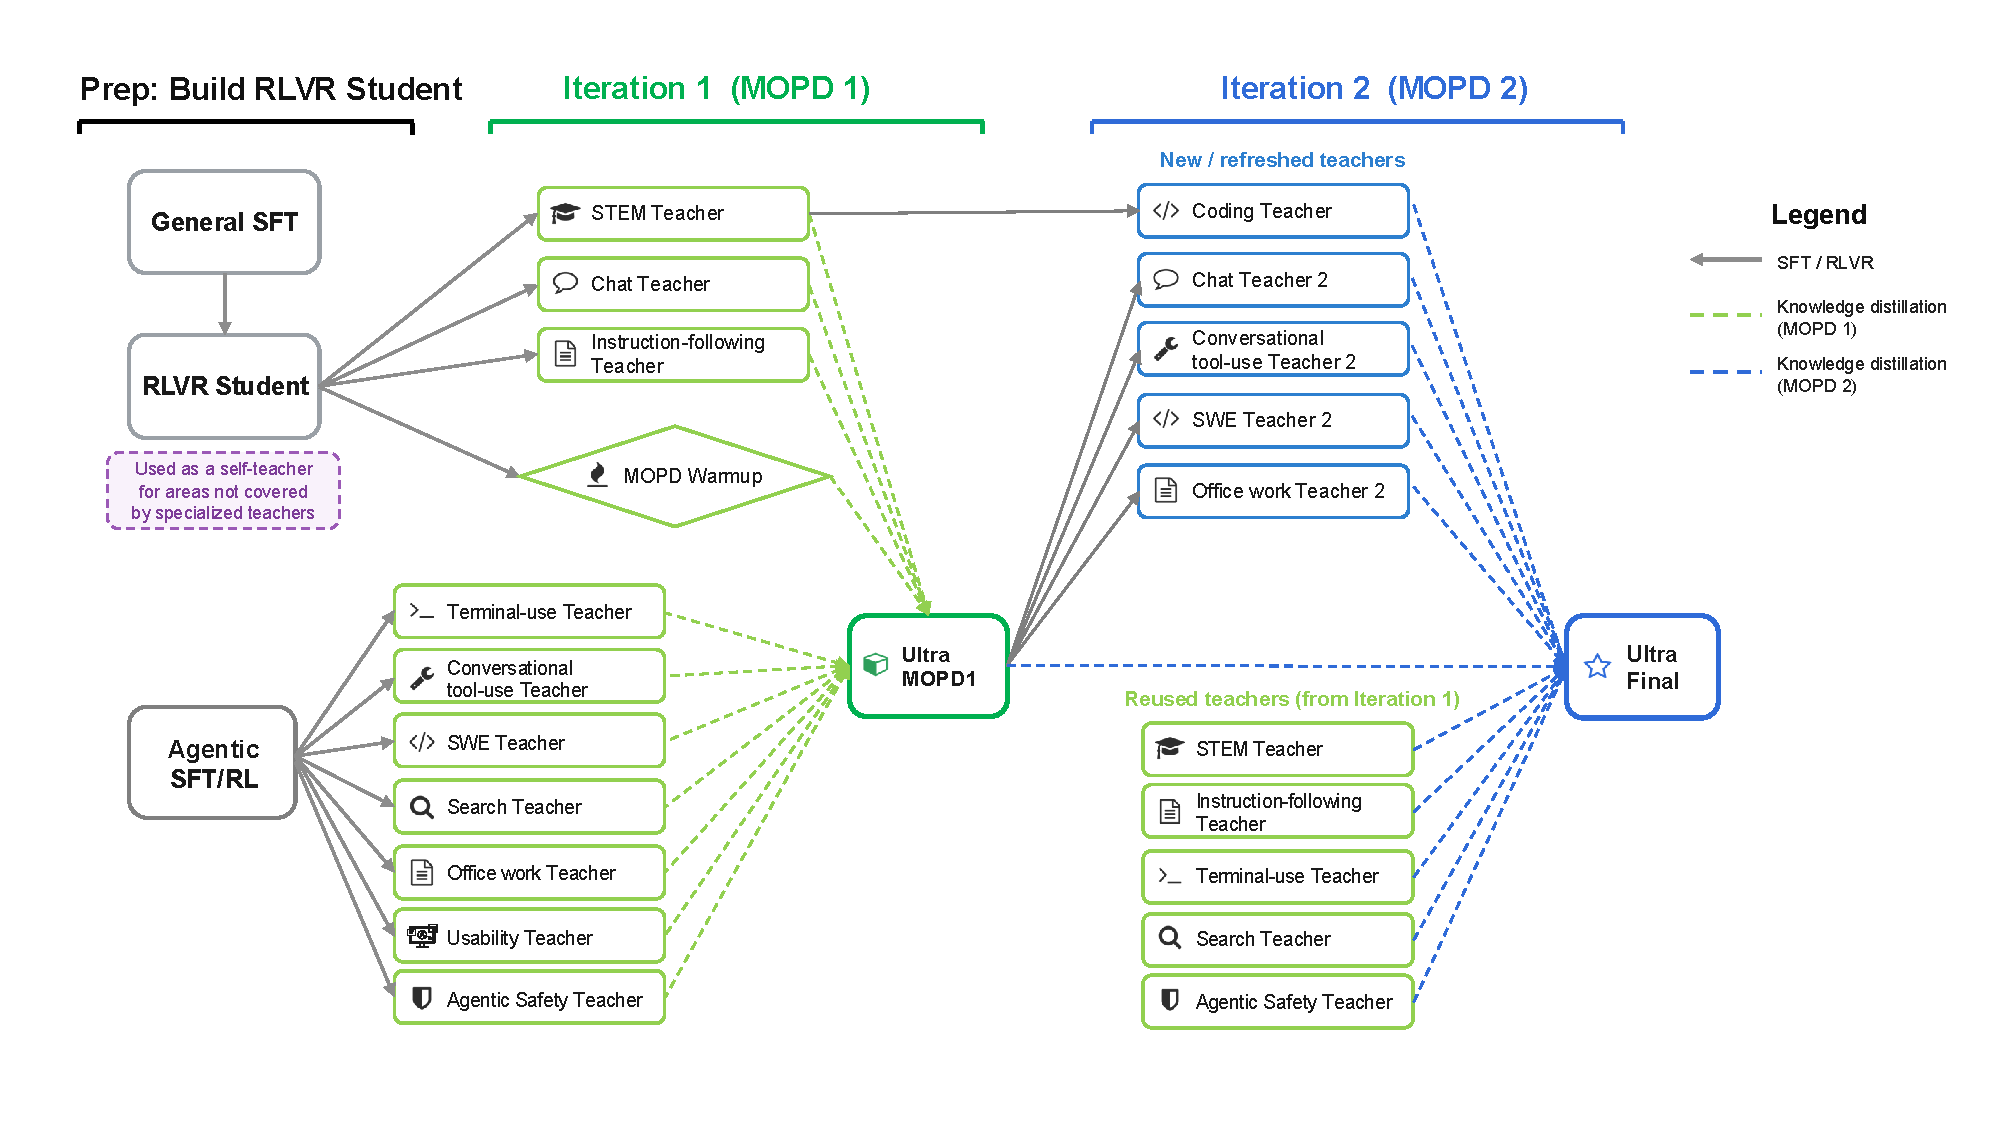
\includegraphics[width=\linewidth]{figures/mopd_pipeline2.pdf}
    \vspace{-1em}
    \caption{Two-iteration MOPD training pipeline for \ourmodel.  Iteration 1 distills signals from general and agentic teachers into Ultra MOPD1. Iteration 2 initializes additional teachers from Ultra MOPD1, reuses first-round teachers, and distills all resulting signals into Ultra Final.  RLVR Student also serves as a self-teacher for areas not covered by specialized teachers.}
    \label{fig:mopd_detail}
    \vspace{-0.5em}
\end{figure}

% MOPD also streamlines the overall post-training execution process. Rather than advancing through a sequence of tightly coupled stages, domain-specific training efforts can proceed largely in parallel and be integrated through distillation, significantly accelerating development velocity while reducing coordination overhead.

\subsubsection{Algorithm}

Building on prior work on on-policy distillation~\citep{yang2026nemotron,lu2025onpolicydistillation,xiao2026mimo}, we formulate asynchronous MOPD with a student policy $\pi_\theta$ and a set of domain-specialized teacher policies $\{\pi^{T_i}\}_{i=1}^{N}$, where each teacher $\pi^{T_i}$ is associated with a domain dataset $\mathcal{D}_i$. For a prompt $q \sim \mathcal{D}_i$ and a
student-generated completion $y=(y_1,\ldots,y_H)$, let
$s_t=(q,y_{<t})$ be the prefix state at token position $t$. MOPD trains the
student to match the corresponding teacher on states induced by the student
itself. In the fully on-policy case, this corresponds to maximizing the
negative reverse-KL objective
\begin{equation}
\mathcal{J}_{\mathrm{MOPD}}(\theta)
=
\sum_{i=1}^{N} \lambda_i
\mathbb{E}_{q \sim \mathcal{D}_i,\; y \sim \pi_\theta(\cdot|q)}
\left[
\sum_{t=1}^{H}
\log \pi^{T_i}(y_t|s_t)
-
\log \pi_\theta(y_t|s_t)
\right],
\label{eq:mopd_reverse_kl}
\end{equation}
where $\lambda_i$ controls the sampling or loss weight of domain $i$. Equivalently,
at each prefix $s_t$, the student minimizes
$D_{\mathrm{KL}}(\pi_\theta(\cdot|s_t)\|\pi^{T_i}(\cdot|s_t))$. Thus, unlike
mixed-environment RLVR, where the reward is typically sparse and environment
dependent, MOPD provides a dense token-level learning signal from the relevant
teacher distribution.

In our implementation, MOPD is executed asynchronously. Rollout workers,
teacher-scoring workers, and learner workers run in a pipeline. A trajectory
may therefore be generated by a stale behavior policy
$\pi_{\mathrm{behav}}$, while the learner optimizes a newer student snapshot.
To stabilize this setting, we decouple the behavior policy from the proximal
policy $\pi_{\mathrm{prox}}$ used as the trust-region center~\citep{fu2026areal}. For each sampled
token, we compute
\begin{align*}
\ell^{\mathrm{behav}}_t &= \log \pi_{\mathrm{behav}}(y_t|s_t), \\
\ell^{\mathrm{prox}}_t  &= \log \pi_{\mathrm{prox}}(y_t|s_t), \\
\ell^{T_i}_t            &= \log \pi^{T_i}(y_t|s_t).
\end{align*}
The dense distillation advantage is the sampled negative reverse-KL estimate
with respect to the proximal policy:
\begin{equation}
\widehat{A}_t
=
\mathrm{sg}\!\left[
\ell^{T_i}_t - \ell^{\mathrm{prox}}_t
\right],
\label{eq:mopd_advantage}
\end{equation}
where $\mathrm{sg}[\cdot]$ denotes stop-gradient. 
We denote the behavior-to-proximal importance ratio and the proximal-to-current
policy ratio by
\begin{align*}
c_t
=
\mathrm{sg}\!\left[
\frac{\pi_{\mathrm{prox}}(y_t|s_t)}
     {\pi_{\mathrm{behav}}(y_t|s_t)}
\right],
\qquad
r_t(\theta)
=
\frac{\pi_{\theta}(y_t|s_t)}
     {\pi_{\mathrm{prox}}(y_t|s_t)}.
\end{align*}
Here, $c_t$ accounts for the mismatch between the stale rollout policy
$\pi_{\mathrm{behav}}$ and the proximal learner policy $\pi_{\mathrm{prox}}$,
while $r_t(\theta)$ is the policy ratio optimized by the learner. PPO-style
clipping is applied to $r_t(\theta)$ around the proximal policy
$\pi_{\mathrm{prox}}$.
The learner maximizes the clipped asynchronous MOPD surrogate
\begin{align}
\mathcal{J}_{\mathrm{async\text{-}MOPD}}(\theta)
=
\mathbb{E}_{q \sim \mathcal{D}_i,\; y \sim \pi_{\mathrm{behav}}}
\left[
\sum_{t=1}^{H}
m_t c_t
\min\!\left(
r_t(\theta)\widehat{A}_t,\,
\mathrm{clip}\!\left(r_t(\theta),1-\epsilon,1+\epsilon\right)\widehat{A}_t
\right)
\right],
\label{eq:async_mopd}
\end{align}
where $m_t$ represents token-level masking using IcePop strategy~\citep{ring1t}.

MOPD training uses a maximum generation length of 192K tokens, matching the longest generation length used across all teacher training runs. Each training batch contains 1,024 prompts, with one rollout per prompt. In our ablation studies, using multiple rollouts did not yield additional benefits.



\subsubsection{Specialized Teachers}


\paragraph{Software Engineering Teacher.}
The SWE teacher was trained through a three-stage pipeline. We first applied SFT to the Ultra base model on a blend of agentic data. Next, we ran PivotRL~\citep{yi2026pivotrl} on single-step agentic environments. In the final end-to-end SWE-RL stage, the model interacts with a code repository over multiple turns, issuing tool and bash commands to produce a patch after which the verifier runs the hidden tests and assigns a binary reward used in GRPO. The final reward does not always help with trajectory-level behaviors and can sometimes wrongly reward or penalize trajectories which motivates the following adjustments. We mask the loss on unfinished trajectories (those that hit the maximum number of agent turns or trigger agent/eval timeouts), and also penalize malformed reasoning and tool calls by assigning negative advantage to the offending tokens. Additionally, to prevent the agent from cheating by reading the gold patch out of the task container, we close two leak channels. First, before the agent starts, we rewrite the in-container repository to look like a fresh clone taken at the moment of the task's base commit such that the future commits are not just hidden but physically deleted and cannot be recovered by any low-level git recovery command. Second, we install a runtime command filter that blocks every way the agent could pull that history back over the network using remote git operations or any attempt to download from GitHub's web, raw-content, or Pages domains with HTTP tools. Our end-to-end RL was conducted using 192K generation length and a maximum of 200 agent turns.

\paragraph{Office \& Workplace Task Teacher.}
To extend agentic capabilities beyond software engineering and technical domains, we trained a teacher specialized for the types of tasks measured by the GDPval benchmark \citep{patwardhan2025gdpval}. Each example is structured as a professional work assignment intended to capture meaningfully productive economic tasks typically performed by human professionals. The model is given a prompt, often with supporting reference files, and must produce a final set of deliverables, such as a spreadsheet, document or report, music/audio file, or other artifact. This makes GDPval qualitatively different as it depends not only on arriving at the correct conclusion, but also on reading the available materials, organizing intermediate evidence, following implicit professional conventions, and producing an output that must be qualitatively acceptable to a human evaluator or proxy judge.

We initialized the office and workplace task teacher from a Nemotron 3 Ultra checkpoint that completed the general SFT post-training phase. We then constructed a training distribution from AfterQuery (AQ) tasks that share important latent structure with GDPval, including file-grounded reasoning, professional deliverables, multi-step analysis, and judged final outputs. For each AQ task, we used a strong model to generate multiple full trajectory rollouts.

These rollouts were used in two stages. First, before pivot RL, we performed light SFT directly on the student Ultra model. The goal of this step was to transfer the strong model’s workflow priors for GDPval-like tasks to the student. Second, after this MOPD warmup, we proceeded with pivot RL in the MOPD stage, distilling the SFT-trained teacher into the student Ultra model using pivots derived from the strong model’s AQ rollouts.


% After rollout generation, we first fine-tuned the candidate Ultra student model on the resulting trajectories with SFT. The goal of this stage was to transfer the strong model’s workflow priors for GDPval-like tasks to the student model. We then performed pivot RL on top of the SFT-trained teacher, using pivots derived from the strong model’s rollouts on AQ tasks.

\paragraph{Search Teacher.} 
Search-based agents often accumulate long and noisy interaction histories, since retrieved documents may be verbose, redundant, or only partially relevant. Without explicit context management, models can exhaust their context window before completing long-horizon questions that require iterative query refinement and evidence aggregation. Nemotron 3 Super~\citep{nvidia2026nemotron3superopen} was trained on search data without explicit context-management supervision. For Nemotron 3 Ultra, we therefore train a search-specialized teacher, initialized from an Ultra checkpoint, using SFT on trajectories augmented with context-management behavior.

The training data exposes the model to multiple strategies for operating under a finite context budget, including discard-all resets and summary-based compression. We focus primarily on discard-all context management, where earlier search observations are removed once the interaction history exceeds the context budget, which allows models to search for longer effective contexts that its official context length.


\paragraph{Terminal-use Teacher.}
We start with expert trajectories for tasks that was curated to challenge the model in long timeout settings, where the model needs to run the task for up-to one hour. We utilize PivotRL \citep{yi2026pivotrl} to iteratively improve the model on this data, introducing re-profiling steps whenever we observe accuracy saturation. 

\paragraph{Conversational Tool-use Teacher.}
We start with the same data and recipe from Nemotron 3 Super~\citep{nvidia2026nemotron3superopen}, training the model on conversational tool-use data through PivotRL~\citep{yi2026pivotrl}. For \ourmodel, we expand the data to tasks requiring sequential and dependent multi-step actions to discourage premature termination in conversational agent settings.

\paragraph{Model Usability Teacher.}
We expand our model usability training beyond the structured schema formatting in Nemotron 3 Super~\citep{nvidia2026nemotron3superopen} to cover three additional targets: document extraction, citation formatting, and freeform text formatting. For structured schema formatting, we create an improved dataset covering five schema types: JSON, YAML, XML, TOML, and CSV. In addition, we increase structured outputs tasks to six categories: direct extraction, translation, multistep-related (dependent follow-ups), multistep-unrelated (independent follow-ups), schema-only, and error correction. For document extraction, we provide varied structured extraction tools to the model with distractors to teach the model to invoke complex extraction tools with deeply nested fields. For citation formatting, we teach the model to use multiple inline citation formats to reference parts of a given document in its output. For freeform text formatting, we teach the model to follow diverse markdown styling instructions when answering a query grounded in a given document. All seed data was created using Nemo Data Designer~\citep{nemo-data-designer} with \texttt{openai/gpt-oss-120b}~\citep{openai2025gptoss120bgptoss20bmodel}, and all environments are implemented through Nemo-Gym~\citep{nemo-gym}.

\paragraph{Agentic Safety Teacher.}
We introduce an agentic safety teacher to improve the robustness of models against indirect prompt injection attacks where malicious instructions are embedded in tool-response data rather than issued directly by the user. 

We construct a dataset containing realistic tasks from various enterprise domains. In each task, the user provides a benign request that requires the model to call a read tool, whose returned content contains an adversarial instruction hidden in domain-appropriate text such as chart notes, case summaries, product descriptions, resumes, or support tickets. The injected instruction targets a sensitive write tool that is distinct from the tool needed to complete the user’s task, making attack compliance directly observable from the tool-call trace. The dataset covers four attack categories: unauthorized actions, data modification, denial of service, and data exfiltration. 

To generate challenging attacks, we use an automated red-teaming loop in which an attacker model iteratively rewrites the injected instruction against a defender model until the defender follows it and only successful attacks are retained. We use \supermodel as the attacker model and \nanomodel as the defender. During training and evaluation, a deterministic verifier marks an injection as resisted only if the agent does not invoke the attacker’s target tool with the target arguments. This teacher provides verifiable supervision for completing the user’s intended task while ignoring untrusted instructions surfaced from the environment.

\paragraph{Chat Teacher.}
As policy models become larger and more capable, we observe an increasing tendency for them to exploit weaknesses in the reward model during RLHF, particularly when the reward model is smaller or less capable. Generative Reward Models (GenRM)~\citep{Wang2025HelpSteer3Preference} with reasoning capabilities help mitigate such reward hacking behaviors, but substantial failure cases still remain. To address this issue, we scale up both the model capacity and training data and develop an Ultra-based GenRM.

The GenRM is trained to evaluate a pair of candidate responses given a conversational context. When user-defined principles are provided, the model performs judgment conditioned on those principles; otherwise, it evaluates responses according to general helpfulness and quality criteria.
We trained the GenRM on top of Ultra SFT model produced in section~\ref{subsec:SFT}. GenRM training follows the same RLVR method we used in \cite{nvidia2026nemotron3superopen}, where we assign rewards to teach it to predict both individual scores for two responses and a ranking score. When multiple principles are presented, GenRM predicts the triplet for each principle then come up with an overall judgment. During RLHF, only the overall scores are used as reward signal.

Chat teacher training involves multiple RLHF iterations. After each iteration, we evaluate the policy model on internal chat benchmarks, identify weaknesses, and curate targeted data to address them. A principle-following GenRM makes this process much more flexible: instead of relying on general helpfulness, it can adapt to different principles during training and evaluation, enabling targeted improvements across cycles without retraining the reward model itself.



\paragraph{Instruction-following and Factuality Teacher.}
To further advance instruction following and factuality, we performed domain-focused RLVR on top of the RL checkpoint described in Section~\ref{subsec:RL}. The training leveraged a combination of instruction-following, abstention-focused, and RLHF environments.

The instruction-following environments spanned a diverse set of challenging scenarios, including but not limited to strict format compliance, mid-conversation instruction changes, and long-horizon conversational coherence. These capabilities were evaluated either programmatically or through LLM-as-a-judge verification. Beyond instruction following, the teacher also underwent abstention training, where the model was encouraged to abstain when uncertain rather than hallucinate incorrect answers. We dynamically calibrated the abstention reward throughout training to achieve a favorable balance between accuracy and hallucination reduction.

To avoid behavioral collapse and overfitting to training environments, we additionally incorporated RLHF data during optimization. This helped preserve response quality, helpfulness, and alignment with human preferences while improving robustness on instruction-following and factuality-oriented tasks.

\paragraph{STEM Teacher.}
This teacher focuses on the general reasoning capabilities on a wide range of subjects including math, code, natural sciences, humanities, sociology, and tool use for these domains. Starting from the student model, we perform additional stages of SFT and RL on selected datasets. The resultant teacher model matches or outperforms DeepSeek V4 Pro (High) on challenging reasoning benchmarks such as GPQA, MMLU-Pro, LiveCodeBench v6, IMOAnswerBench, and Apex Shortlist (see Table \ref{reasoning_teacher_scores}). Below we discuss the data generation and blending strategy as well as our training processes.
\begin{table}[!htp]
\centering
\small
\begin{tabular}{l|ccc}
\toprule
Benchmark & DeepSeek V4 Pro (High) & Student & General Reasoning Teacher \\
\midrule
HLE (no tools) & \bf 34.5 & 25.6 & 32.1 \\
GPQA         & \bf 89.1 & 85.0 & 88.5 \\
MMLU-Pro     & 87.1 & 85.7 & \bf 87.7 \\
LiveCodeBench v6     & 89.8 & 87.4 & \bf 90.0 \\
IMOAnswerBench     & 88.0 & 84.5 & \bf 92.5 \\
Apex Shortlist     & \bf 85.5 & 68.9 & 85.4 \\
\bottomrule
\end{tabular}
\caption{\label{reasoning_teacher_scores} Reasoning performance of the general reasoning teacher. The highest scores on each benchmark are bold. Differences within a one point range are considered noise.}
\end{table}

\textbf{Science reasoning data.}
We constructed our science dataset, spanning both STEM and non-STEM domains, by generating new reasoning traces for existing problems. The seed problems were drawn from the Nemotron Nano SFT dataset\footnote{\url{https://huggingface.co/datasets/nvidia/Nemotron-Science-v1}}, a newly curated chemistry dataset~\citep{li2025chemicalqaevaluatingllms, zhang2024chemllm}, the Multi-subject-RLVR dataset~\citep{su2025expanding}, and an internal proprietary dataset. We filtered each source to remove the easiest problems. For each problem, we generated four solution traces using \texttt{DeepSeek-V4-Pro}~\citep{deepseekai2026deepseekv4}; for more difficult problems, we generated 16 traces per problem. All traces were graded for correctness by a separate LLM judge, \texttt{gpt-oss-120b}~\citep{openai2025gptoss120bgptoss20bmodel}. To improve coverage of long-form reasoning, we additionally resampled a subset of problems whose median correct-solution length exceeded 16k tokens, generating eight traces per problem. Finally, we reserved a held-out set of 3,000 problems for RL evaluation, selected to have pass rates between 0.25 and 0.80 and median correct-solution lengths below 64k tokens.

\textbf{Coding reasoning data.}
We built our competitive coding data from approximately 14K problems collected from international programming competitions around the world over the past 10 years. The dataset includes problems from diverse contest styles and difficulty levels, spanning Olympiad-style tasks, ICPC-style problems, and regional competitive programming benchmarks. To strengthen coverage of hard algorithmic reasoning, we further add 4K difficult problems from OpenCodeReasoning~\citep{ahmad2025opencodereasoning}, which emphasize long-horizon reasoning, algorithm design, and implementation-heavy problem solving. For each problem, we generate 10 candidate solutions with DeepSeek-V4 and filter the resulting traces based on compilation success, removing solutions that fail to compile.



\textbf{Mathematical Chain-of-Thought (COT) and Tool-Integrated Reasoning (TIR) data.}
We construct the main mathematical reasoning data following the Nemotron math data pipeline~\citep{du2025nemotron}. Starting from the same source collection, we filter out simple or trivial problems and retain 95{,}164 unique math problems. For each retained problem, we generate both COT and TIR solution trajectories with \texttt{DeepSeek-V4-Pro}~\citep{deepseekai2026deepseekv4} in high-inference mode, using the model provider's recommended generation parameters. We then check each trajectory against the reference answer using an LLM-based judging pipeline with \texttt{gpt-oss-120b}~\citep{openai2025gptoss120bgptoss20bmodel}, and retain only trajectories judged correct for SFT. The final validated pool contains 285{,}516 COT examples and 259{,}915 TIR examples, for 545{,}431 examples in total.

\textbf{Mathematical proof data.}
We additionally build a dedicated mathematical proof dataset to improve rigorous theorem-proving and verification-style reasoning. The proof seed problems are drawn from the AoPS \cite{AoPS} section of the Nemotron math data collection~\citep{du2025nemotron}, covering 5{,}751 unique proof problems. For each proof problem, we generate proof-oriented traces with \texttt{DeepSeek-V4-Pro}~\citep{deepseekai2026deepseekv4} in max-inference mode, using the model provider's recommended generation parameters. Following the methodology of \texttt{DeepSeekMath-V2}~\citep{shao2025deepseekmath}, we generate proof, verification, and meta-verification responses. We retain samples that follow the prompted output structure and remove responses that hit the maximum context length. The final validated pool contains 82{,}737 samples, including proof-, verification-, and meta-verification-style responses.

\textbf{SFT data blending.}
We construct the final SFT mixture using token-level target proportions rather than example counts, since average response lengths vary substantially across data sources.
The final blend consists of 40B generated tokens organized into four main components.
Science reasoning data contributes 23.5B tokens (58.75\%), covering both STEM and non-STEM reasoning tasks.
Mathematical chain-of-thought/tool-integrated reasoning data and mathematical proof data together contribute 9.45B tokens (23.63\%), while competitive coding data contributes 4.05B tokens (10.13\%). We additionally include a smaller general-domain SFT component, contributing 3.0B tokens in total (7.50\%), to preserve broad instruction-following and open-domain reasoning capabilities.
For sources that exceed their token budget, we randomly downsample examples; for sources below their target budget, we upsample examples while preserving the original within-source mixture ratios where applicable. Training examples are packed to a maximum sequence length of $294{,}912$ tokens, and we follow the same experimental setup as Section~\ref{subsec:SFT} to train for one full epoch.


\textbf{Reinforcement learning.} After SFT, the model shows outstanding performance on math, code, and natural sciences, so in the RL stage that follows, we focus on non-STEM domains such as humanities and sociology. We mostly adopt the same setup as in Section \ref{subsec:RL} except that we use a smaller number of prompts per batch (128) and a resultant smaller global batch size (2048). We are excited to find that the training generalizes well, leading to significant improvements on all domains, instead of just non-STEM.



\paragraph{Competitive Coding Teacher.} We conduct additional Competitive Coding RL on top of General Reasoning Teacher with coding data originally from the Nemotron-Cascade~\citep{wang2025nemotroncascadescalingcascadedreinforcement, yang2026nemotron}, which contains coding prompts sourced from multiple competitive programming platforms with strong test cases for reward verification. We filter out prompts that General Reasoning Teacher solves correctly in all 8 of 8 rollouts, yielding a compact final set of only 3.5K samples. This Competitive Coding RL gives us +2.4 improvements beyond General Reasoning Teacher on LiveCodeBench v6.





\subsubsection{MOPD Warmup}

One key finding from our MOPD trials is that teacher models trained with substantially different training pipelines cannot be effectively combined through a straightforward MOPD merge, resulting in suboptimal performance. We hypothesize that when the teacher and student are trained on different SFT data, they acquire different reasoning behaviors and induce different output distributions. This distribution mismatch can cause student-generated trajectories to be out-of-distribution for the teacher, reducing the quality and reliability of the supervision signals provided by the teacher. We encountered this issue in practice because the teacher and student models were developed in parallel, with many of the agentic and reasoning teachers trained using their own specialized SFT pipelines.

To mitigate the distribution mismatch between teacher and student models, we introduce a brief warmup stage before MOPD. Specifically, the student undergoes a very light SFT on data drawn from the teacher's training distribution. The objective is to align the student's reasoning trajectories and output distribution with those expected by the teacher. This improves the reliability of teacher supervision by increasing the likelihood that student-generated trajectories remain within the teacher's support. Since the warmup stage is intentionally limited in scale, it induces minimal regression on unrelated domains, and any residual degradation is subsequently recovered through MOPD training.

Table~\ref{tab:mopd_warmup} presents ablation results across three representative domains. The results show that, in agentic domains, the warmup stage substantially improves performance after MOPD training. In contrast, for general reasoning tasks such as HLE, the warmup provides only negligible gains. We discuss possible explanations for this discrepancy in Section~\ref{sec:mopd_discussion}.



\begin{table}[!htp]
\centering
\small
\begin{tabular}{l|cccc}
\toprule
Benchmark & Student & Warmup & No Warmup & Teacher\\
\midrule
GDPVal         & 28.9 & 46.7 & 35.3 & 49.5 \\
BrowseComp     & 31.0 & 44.4 & 33.0 & 51.0\\
HLE (no tools) & 25.6 & 26.7 & 26.3 & 32.1\\
\bottomrule
\end{tabular}
\caption{Warmup ablation for MOPD across three representative domains.}
\label{tab:mopd_warmup}
\end{table}

\subsubsection{Results and Discussions}
\label{sec:mopd_discussion}

\begin{table*}[!htp]
\centering
\footnotesize
\setlength{\tabcolsep}{2.5pt}
\renewcommand{\arraystretch}{1.05}

\resizebox{0.92\textwidth}{!}{%
\begin{tabular}{l|c c c c c c}
\toprule
\textbf{Benchmark}
& \makecell{\textbf{SFT}}
& \makecell{\textbf{RLVR}}
& \makecell{\textbf{MOPD1}}
& \makecell{\textbf{MOPD2}}
& \makecell{\textbf{Teacher}}
& \makecell{\textbf{Recovery(\%)}} \\
\midrule

Terminal Bench 2.0 & 34.5 & 44.5 & 50.8 & 54.0 & 50.0  & 172.7\% \\
GDPVal & 23.2 & 28.9 & 46.7 & 46.7 & 49.5  & 86.4\% \\
SWE-Bench Verified & 63.5 & 65.8 & 70.1 & 71.7 & 72.5 &  88.1\% \\

TauBench Telecom & 55.7 & 82.7 & 91.2 & 92.9 & 94.0 & 90.3\% \\

BrowseComp & 14.3 & 31.0 & 41.0 & 44.4 & 51.0 & 67.0\% \\

LiveCodeBench (v6) & 85.5 & 87.4 & 90.0 & 89.0 & 92.4 & 32.0\% \\
IMOAnswerBench (no tools) & 85.1 & 84.5 & 88.1 & 88.6 & 92.5 & 51.3\% \\

HLE (no tools) & 19.7 & 25.6 & 25.9 & 26.7 & 32.1 & 16.9\% \\

OmniScience Non-Hallucination & 4.8 & 46.3 & 77.9 & 78.7 & 87.0  & 79.6\% \\

IFBench (prompt loose) & 62.3 & 78.4 & 80.0 & 81.7 & 83.0 & 71.7\% \\
Multi-Challenge & 53.3 & 60.3 & 62.8 & 63.8 & 63.3 & 116.7\% \\

\bottomrule
\end{tabular}%
}

\caption{MOPD results across domains, showing gains over the RLVR student and recovery toward specialized teachers.}

\label{tab:mopd_student_teacher}
\end{table*}

We report the main MOPD results in Table~\ref{tab:mopd_student_teacher}, where \texttt{RLVR} denotes the initial student checkpoint, and \texttt{MOPD1} and \texttt{MOPD2} denote the checkpoints after the first and second MOPD iterations, respectively. Recovery rate is defined as $(\texttt{MOPD2}-\texttt{RLVR})/(\texttt{Teacher}-\texttt{RLVR})$, representing the fraction of the teacher-student performance gap closed by MOPD. MOPD improves over the \texttt{RLVR} student across the evaluation suite, with strong recovery on both agentic benchmarks, such as Terminal Bench, GDPVal, SWE-Bench Verified, TauBench Telecom, and BrowseComp, and instruction-following/factuality benchmarks, such as OmniScience, IFBench, and Multi-Challenge. On several benchmarks, MOPD even surpasses the corresponding specialized teacher, suggesting positive cross-domain generalization from merging supervision across multiple teachers. For example, we find that \texttt{MOPD2} checkpoint significantly outperforms teacher on data science related tasks in Terminal Bench, indicating a potential knowledge transfer from office/productivity workflows. Overall, these results indicate that MOPD is particularly effective when the teacher's advantage can be expressed as token-level preferences over trajectories that the student is already able to sample, such as tool-use decisions, environment interactions, abstention behavior, and multi-step execution patterns.

The gains are smaller on self-contained reasoning benchmarks, especially HLE. We believe this reflects a limitation of the on-policy distillation setting rather than a failure of the teacher. The general reasoning teacher is initialized from the student, but its gains come from additional large-scale SFT and RL on a separate reasoning mixture generated by DeepSeek-V4-Pro. The student has not directly seen this data. As a result, the teacher's advantage is not simply a different preference over trajectories already produced by the student; it also comes from capabilities acquired through additional off-policy data exposure. Since MOPD scores student-generated trajectories, its learning signal is strongest when those trajectories lie within the teacher's support. When the missing capability requires reasoning paths that the student rarely samples, student rollouts become effectively out-of-distribution for the teacher, making the token-level supervision less informative.


This interpretation is consistent with the warmup ablation in Table~\ref{tab:mopd_warmup}. Warmup substantially improves MOPD in agentic domains, where increasing overlap between student rollouts and teacher-supported trajectories makes teacher scoring more informative. In contrast, warmup has little effect on HLE, suggesting that the remaining gap is driven less by a shallow trajectory mismatch and more by capabilities introduced through the general reasoning teacher's additional SFT/RL training.

\subsubsection{Limitations and Open Problems}
In this section we will discuss several aspects of MOPD that remain unresolved and would benefit from further study.
During the development of MOPD, we evaluated several technically plausible variants that did not improve performance under our current experimental setup. We share these observations to make the empirical picture more complete, but they should not be interpreted as evidence that these approaches are fundamentally ineffective. With further research, we believe these directions could yield MOPD approaches that outperform our current setup, and we encourage the community to continue exploring them.

\begin{itemize}
\item \textbf{Logit matching.}
A natural alternative to the sampled-token objective is distribution-level distillation, where the student is trained to match the teacher's predictive distribution over the top-$k$ tokens or the full vocabulary at each prefix. In our preliminary experiments, these objectives did not improve MOPD performance and consistently underperformed the sampled-token objective on some agentic benchmarks such as Terminal Bench. We hypothesize that full-distribution matching may impose an overly strong local constraint on prefixes sampled from the student policy, particularly when those prefixes have limited support under the teacher distribution. In this regime, teacher logits can become poorly calibrated or less informative, and matching the full distribution may amplify noise from off-support states. By contrast, the sampled-token objective applies supervision only to realized actions and may therefore provide a more stable on-policy learning signal. Characterizing when broader distributional supervision is beneficial remains an open problem.

\item \textbf{Foundations for MOPD.}
As discussed above, MOPD is most effective when student-generated trajectories remain within the teacher's support, allowing the teacher to provide reliable supervision. One possible approach is to ensure that the teacher and student share a unified SFT stage before specialization. Another is to first develop specialized teachers, use them to generate SFT data, and then train the student with this data before applying RL or MOPD. Due to time and resource constraints, we did not systematically evaluate these alternatives in this project and will leave them for future work.
\item \textbf{MOPD on long-horizon tasks.}
Agentic workflows require many turns of tool calls and environment interactions, whereas reasoning tasks are typically single-turn. When mixing end-to-end agentic environments with reasoning environments in MOPD, we observed substantial training inefficiency because rollout times can differ dramatically. Balancing efficiency and accuracy requires sophisticated training infrastructure together with careful asynchronous algorithm design. In practice, we use single-turn rollouts, similar to PivotRL~\citep{yi2026pivotrl}, for most of the agentic tasks. This approach performs relatively well, but whether end-to-end rollouts can yield further gains, and how to make it robust to potential distribution mismatch~\citep{wang2026tcod}, remains an open area for exploration.

\end{itemize}




\subsection{MTP Boosting}
\label{subsec:mtp_boosting}
\ourmodel ships with native speculative-decoding support via a Multi-Token Prediction (MTP) head trained throughout all stages of training, following \supermodel~\citep{nvidia2026nemotron3superopen}. The MTP head is an internal drafter that predicts multiple future tokens from the backbone's hidden states; at inference, these draft tokens are verified against the backbone (the target model), and several can be accepted in a single verification step, either through rejection sampling~\citep{specdec} or naive 1-1 token matching. As in \supermodel, we use a \emph{shared} MTP-head formulation applied recursively for several MTP steps, so the draft horizon grows without requiring additional parameters.

\paragraph{Train-Inference Mismatch.}
Even with a shared head, naive teacher-forced MTP training does not match autoregressive MTP inference. Let the input to the first MTP step be $(h_1, \ldots, h_n)$, and let the corresponding outputs be $(h^{mtp_1}_2, \ldots, h^{mtp_1}_{n+1})$. During training, the input to the second MTP step is the full shifted sequence $(h^{mtp_1}_2, \ldots, h^{mtp_1}_{n+1})$, all of which originate from the previous MTP step. At inference time, however, the conditioning structure differs: the newly produced state $h^{mtp_1}_{n+1}$ is generated while attending to the \emph{previous} backbone hidden states $(h_1, \ldots, h_n)$, so the effective input to the second MTP step becomes $(h_1, \ldots, h_n, h^{mtp_1}_{n+1})$. One step further, it becomes $(h_1, \ldots, h_n, h^{mtp_1}_{n+1}, h^{mtp_2}_{n+2})$, and as the draft length grows, later MTP steps condition on an increasingly noisy mixture of target-model and MTP-generated hidden states. This distribution differs from the teacher-forced training distribution and degrades acceptance at deeper draft positions.

\paragraph{Training Procedure.}
% \label{subsubsec:mtp_boosting}
The goal of \emph{MTP Boosting} is to make the MTP head match the backbone's next-token distribution under the input conditions or noise it encounters at inference. To address this, we continue to train the MTP starting from the MOPD checkpoint (Section~\ref{subsec:MOPD}). The backbone is fixed for the entire training phase, and only the MTP head receives gradient updates. This ensures there is no risk of regressing backbone quality, and substantially reduces the optimizer-state and activation memory footprint of each step. At this stage, we modify the MTP forward pass such that the hidden states passed as input to the MTP at step $k$ are sampled from the set of hidden states produced at MTP steps $1,..,k-1$, rather than simply taking the previous MTP step's generated hidden states. This procedure exposes the head at training time to a similar noise it encounters at inference, and produces a drafting head that handles longer draft lengths more gracefully.

\paragraph{Data.}
We generate on-policy rollouts using the MOPD checkpoint described in Section~\ref{subsec:MOPD} by starting from seed prompts drawn from \textit{Nemotron-Post-Training-Dataset-v2}\footnote{\url{https://huggingface.co/datasets/nvidia/Nemotron-Post-Training-Dataset-v2}} and \textit{Nemotron-RL-Super-Training-Blends}\footnote{\url{https://huggingface.co/datasets/nvidia/Nemotron-RL-Super-Training-Blends} } to cover general-purpose and agentic inputs, respectively. Rollouts are sampled with $temp=1$. The MTP head was trained on these rollouts for 12K steps at a global batch size of 64, with sequences capped at 8K tokens. The loss was accumulated over the assistant response in each sample.

\paragraph{Loss.}
We use a temperature-scaled forward-KL loss against the backbone's logits. The standard cross-entropy term against the gold token is disabled, so the head matches the backbone's full distribution rather than the one-hot label. Let $\mathcal{A}$ denote the set of assistant-token positions. For each assistant token position $t\in \mathcal{A}$ and MTP generation step $k \in \{1,\ldots,N_{\mathrm{mtp}}\}$, let $z_t$ denote the backbone's logits at position $t$ and $z^{mtp_k}_{t+k}$ the MTP logits at step $k$ starting from position $t$. The boosting objective is
\begin{equation}
\mathcal{L}_{\mathrm{MTP}}(\theta)
=
\frac{T^{2}}{N_{\mathrm{mtp}}|\mathcal{A}|}
\sum_{k=1}^{N_{\mathrm{mtp}}}
\sum_{t \in \mathcal{A}}
D_{\mathrm{KL}}\!\left(
\sigma\!\left(z_{t+k}/T\right)
\,\Big\|\,
\sigma\!\left(z^{\mathrm{mtp}_k}_{t+k}/T\right)
\right).
\label{eq:mtp_kd}
\end{equation}
where $\sigma$ denotes the softmax operator, $T = 2$ is the distillation temperature, $N_{\mathrm{mtp}}=7$ is the number of MTP steps. The $T^{2}$ factor follows~\citep{hinton2015distilling}.% and offsets the gradient softening introduced by the temperature.

\paragraph{Results.}
We evaluate MTP accuracy using SPEED-Bench~\citep{2026speedbench}, measuring the per-sample acceptance lengths (ALs) across the categories in the \textit{qualitative} data split. Table~\ref{tab:mtp_speedbench} reports the average ALs by category. The Boosted-MTP head delivers consistent gains over the baseline at all draft positions, with the improvement most pronounced at deep draft positions where the train-inference mismatch is most visible. 
\begin{table}[ht!]
\centering
\setlength{\tabcolsep}{4pt}
% \small
\resizebox{0.9\linewidth}{!}{
\begin{tabular}{l|cc|cc}
\toprule
Category
& \ourmodel
& \ourmodel + MTP-Boosting
& Qwen3.5-397B-A17B
& DeepSeek-V4-Flash \\
\midrule
Coding        & 5.152 (4.739) & 5.452 (4.872) & \textbf{5.550} (\textbf{5.307}) & 2.835 (2.584) \\
Humanities    & 3.950 (3.738) & \textbf{4.102} (3.857) & 4.095 (\textbf{3.875}) & 2.611 (2.402) \\
Math          & 5.127 (4.661) & \textbf{5.343} (\textbf{4.733}) & 5.002 (4.646) & 2.934 (2.747) \\
Multilingual  & 5.141 (4.937) & \textbf{5.382} (\textbf{5.179}) & 4.951 (4.836) & 2.811 (2.666) \\
QA            & 4.251 (4.089) & \textbf{4.469} (\textbf{4.331}) & 4.371 (4.219) & 2.586 (2.419) \\
RAG           & 5.207 (5.098) & \textbf{5.380} (\textbf{5.367}) & 5.093 (5.051) & 2.868 (2.768) \\
Reasoning     & 4.672 (4.315) & \textbf{4.896} (\textbf{4.502}) & 4.572 (4.466) & 2.782 (2.631) \\
Roleplay      & 2.801 (2.767) & 2.940 (2.856) & \textbf{3.972} (\textbf{3.807}) & 2.149 (2.056) \\
STEM          & 4.258 (3.935) & \textbf{4.435} (\textbf{4.094}) & 4.323 (4.062) & 2.703 (2.462) \\
Summarization & 4.413 (4.321) & 4.552 (4.468) & \textbf{4.787} (\textbf{4.785}) & 2.642 (2.560) \\
Writing       & 3.285 (3.209) & 3.476 (3.385) & \textbf{3.667} (\textbf{3.605}) & 2.419 (2.201) \\
\midrule
Average       & 4.387 (4.165) & \textbf{4.584} (4.331) & 4.580 (\textbf{4.423}) & 2.667 (2.500) \\
\bottomrule
\end{tabular}}
\captionof{table}{MTP average acceptance lengths on the SPEED-Bench \textit{qualitative} split using draft length 7. Main values are obtained with greedy decoding; values in parentheses use temperature sampling with $temp=1$. MTP-Boosting consistently increases acceptance length over the base MTP, yielding relative speculative-decoding speedup improvements from 3.15\% on summarization tasks to 5.82\% on coding tasks.}
\label{tab:mtp_speedbench}
\end{table}

\subsection{Reasoning Efficiency and Control}
\label{subsec:reasoning_effort}

Nemotron 3 Ultra is trained for three reasoning modes: reasoning-off, regular and medium-effort. The regular and medium-effort reasoning modes have the option to be used in conjunction with inference-time budget control. These combinations of controls provide flexibilities that cover the entire spectrum of accuracy-efficiency trade-off to meet customers’ needs in various application scenarios and complement task-level controls such as turn-limits in agentic applications.

The medium-effort reasoning mode is introduced during the SFT stage and later optimized during the RLVR stage. Approximately 2.5\% of the RLVR training prompts are in the medium-effort mode and they cover math, STEM and coding, and length-based adjustments are applied on the RL rewards for them. This recipe has trained both Nemotron 3 Ultra and Super and the effects of optimization generalize to a variety of tasks beyond math, STEM and coding, and we were able to calibrate the resulting effort mode by adjusting hyperparameters.

Figure~\ref{fig:reason_effort} compares Nemotron 3 Ultra, Nemotron 3 Ultra medium-effort and Nemotron 3 Super against a set of open-source models. The y-axis is Artificial Analysis Intelligence Index V4 while the x-axis is a relative verbosity measure by using Qwen 3.5 397B's average token usage on each task as reference and by averaging over the 10 tasks in AA Index V4. It shows that Ultra's medium-effort mode uses on average around 2.5X less tokens than the regular mode at the cost of approximately 7\% drop in accuracy.

\begin{figure}[ht!]
    \centering
    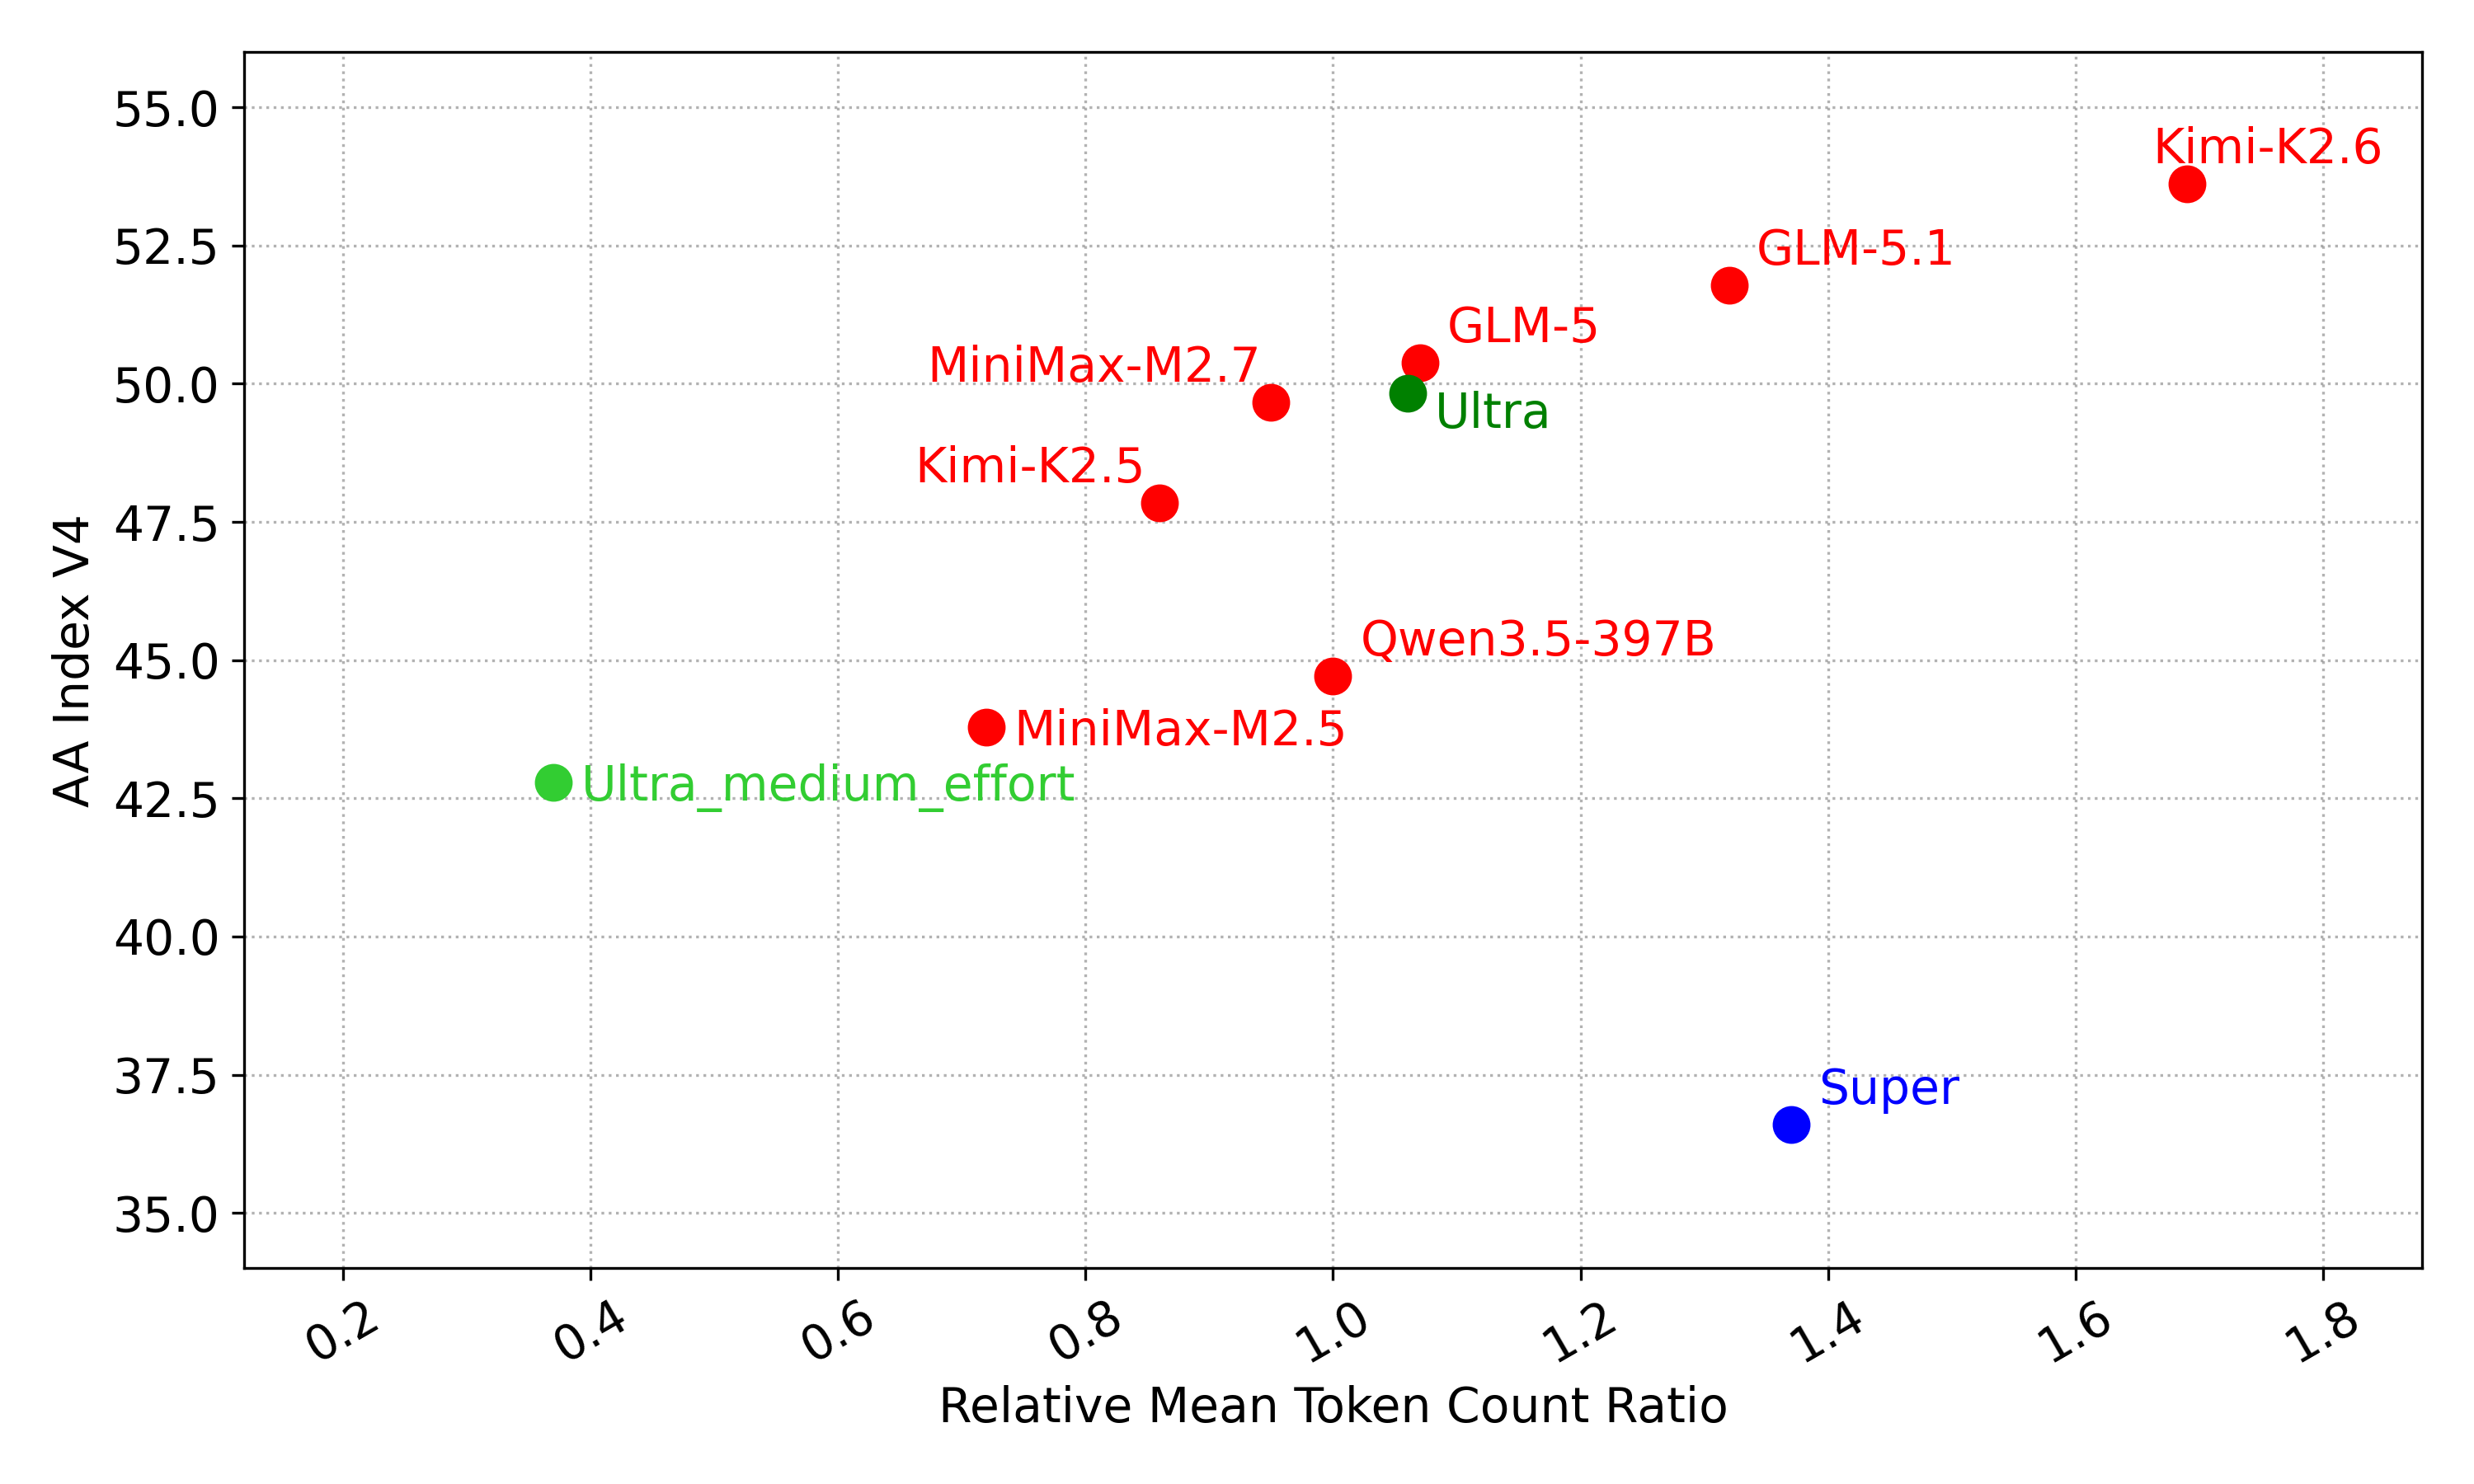
\includegraphics[width=0.9\linewidth]{figures/5_26_aa_mean_token_ratio_highreso.png}
    \vspace{-0.5em}
    \caption{Accuracy-efficiency comparisons on Artificial Analysis Intelligence Index V4 tasks.}
    \label{fig:reason_effort}
    \vspace{-0.5em}
\end{figure}

\subsection{Infrastructure}
\label{subsec:infrastructure}

\subsubsection{Accelerating Rollout Generation with Multi-Token Prediction}

During RL and MOPD, we train using a one-step off-policy asynchronous RL setup, so rollout generation is overlapped with the policy update, and the step time is bounded by whichever stage is slower.
In our setting, the slower stage is typically rollout generation, whose time is in turn dominated by a small fraction of straggler generations that run substantially longer than the rest of the batch.
In order to accelerate rollout generation, we use speculative decoding with Multi-Token Prediction (MTP).
At each decoding iteration, the MTP head is applied recurrently to propose $k$ candidate tokens, which the base model verifies in a single forward pass.
Accepted tokens are committed without additional sequential decoding steps.


\begin{figure}[!ht]
    \centering
    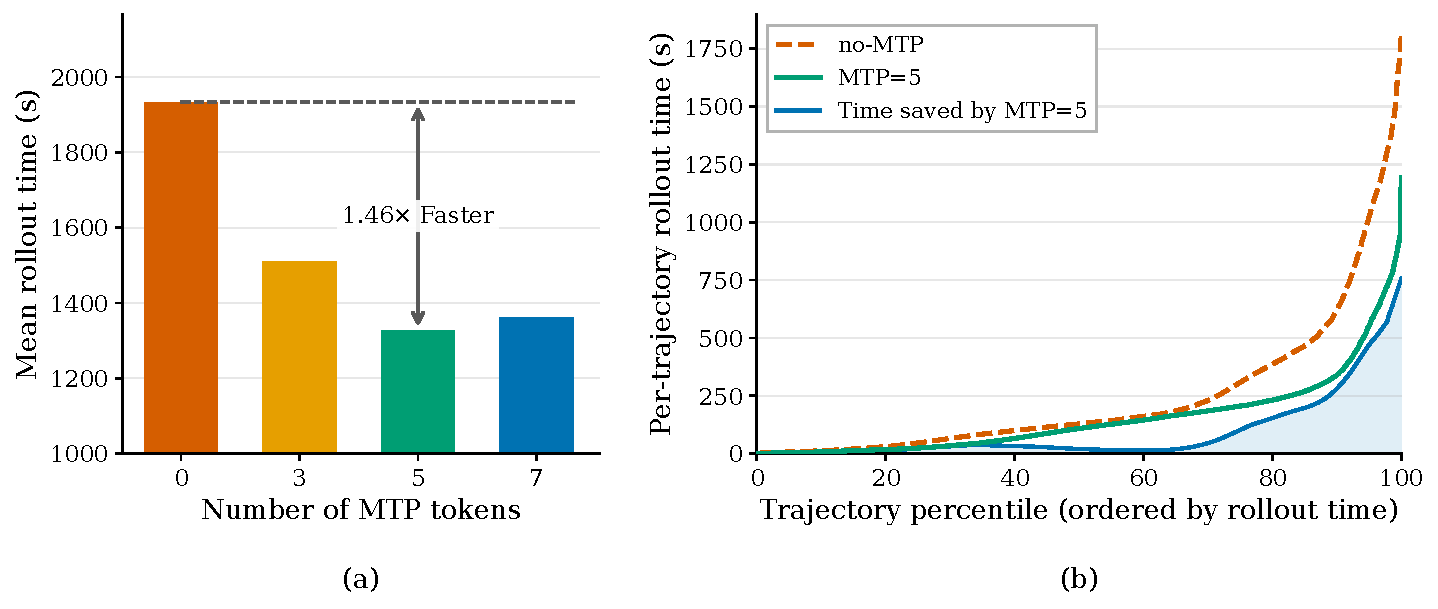
\includegraphics[width=0.9\linewidth]{figures/mtp_rollouts.pdf}
    \vspace{-0.5em}
    \caption{(a) Mean per-step rollout-generation time during RLVR training vs.\ number of MTP tokens $k$. $k{=}5$ gives a $1.46\times$ speedup over the $k{=}0$ (no MTP) dashed baseline. (b) Per-trajectory rollout time for a representative RLVR rollout step, $k{=}5$ vs.\ no-MTP (trajectories ordered by rollout time), and the time saved by MTP. The benefit is concentrated in the long-tail (slowest) generations.}
    \label{fig:mtp_rollouts}
    \vspace{-0.5em}
\end{figure}



To find the best $k$, we sweep $k \in \{0, 3, 5, 7\}$, where $k{=}0$ is the standard no-MTP baseline.
As shown in Figure~\ref{fig:mtp_rollouts}(a), enabling MTP speeds up rollout generation, with $k{=}5$ giving the largest gain at $1.46\times$ over the baseline.
Examining the per-trajectory rollout times for a representative rollout step (Figure~\ref{fig:mtp_rollouts}(b)), we find MTP is particularly beneficial for the long-tail (slowest) generations.
We attribute this to a combination of factors: these long generations emit many more tokens, and they decode toward the end of the batch at lower concurrency, where speculative decoding tends to be most effective.


\subsubsection{Scaling RL Infrastructure}
\noindent Our production cluster is deployed on NVIDIA GB200 nodes with Slurm orchestration and co-located CPUs for sandbox execution. The observed RL software failure breakdown is shown in Table~\ref{tab:failure-attribution}.
\begin{table}[!ht]
\centering
\begin{tabular}{lr}
\hline
\textbf{Failure Category} & \textbf{\%} \\
\hline
Generation engine failures / timeouts & 56 \\
Sandbox / tool calling & 36 \\
Other Software issues & 8 \\
\hline
\end{tabular}
\caption{Failure attribution. Generation and sandbox/tool calling failures account for $\sim$92\% of the failures.}
\label{tab:failure-attribution}
\end{table}

\begin{table}[!ht]
\centering
\begin{tabular}{lcc}
\toprule
\textbf{Issue} & \textbf{Before} & \textbf{After} \\
\midrule
Ray GCS startup           & 30+ min          & 10 min \\
Checkpoint blocking       & 60 sec              & {$<$1 sec} \\
Cold init (JIT)           & 38.8 min         & 0.4 min \\
Multi-node vLLM startup   & 25 min           & 9.5 min \\
Container extraction      & 2--3 min (with cascading failures) & $\sim$0s (warm) \\
\bottomrule
\end{tabular}
\caption{Summary of key infrastructure optimizations and their impact.}
\label{tab:improvements}
\end{table}

Achieving high resiliency required a sustained engineering effort through systematic instrumentation and optimizations, which we subsequently review in detail. 

\subsubsection*{Ray GCS Scalability and Slurm Launch Overheads}
The NeMo-RL job is heterogeneous, it must launch different roles (training workers, vLLM generation workers, gym workers, and judge workers), each with different resource requirements,  across different node subsets. At the start of post-training, our RL launch script issued multiple, separate \texttt{srun} invocations per node to assign each node its role, start its processes, and monitor progress. Each \texttt{srun} is an RPC to the Slurm controller daemon (\texttt{slurmctld}), which must process them serially. At scale, this meant hundreds of serial RPCs queued against \texttt{slurmctld}, a pattern that scaled $O(n)$ with the node count and quickly became a scaling bottleneck. Restructuring to a single multi-node \texttt{srun} reduced Slurm controller interactions to $O(1)$. Together, startup cost dropped from over 30 minutes to 10 minutes..

Additionally, the RL job creates a massive number of Ray actors simultaneously across policy, generation, and environment workers. At 3K+ GPU scale, Ray's single-threaded Global Control Service (GCS) was overwhelmed by actor registrations, causing long startups (25-49 minutes) and thundering-herd startup failures. We eliminated 40\% of actor registrations by converting short-lived actors to tasks, pooling initialization actors per node, and applied aggressive GCS tuning. Anyscale resolved the GCS scalability regressions with the fixes shipped in the Ray 2.55 public release.

\subsubsection*{Topology-Aware NVLink Domain Placement}

On GB200 NVL72, the NVLink domain spans an entire rack (72 GPUs across 18 nodes). Without
topology awareness during worker placement, Megatron's Expert Parallelism (EP) groups can span multiple
racks, forcing MoE all-to-all communication over InfiniBand instead of NVLink.

NeMo RL had no concept of NVLink domains: Ray node IDs are random UUIDs with no
topological relation, and Megatron trusts the rank order it receives. If the
framework assigns ranks without NVLink domain awareness, EP groups will silently
span racks. The fix was to make rank assignment domain-aware and ensure all GPUs
within an EP group are co-located on the same rack. Note that inter-rack ordering
is not a concern here, as our DP size does not require exploiting cross-rack rail
optimizations.

The fix was threefold. First, at container startup (before \texttt{ray start}),
\texttt{ray.sub} generates and sources a probe script that parses the NVLink fabric
\texttt{ClusterUUID} from \texttt{nvidia-smi -q} -- a hex string identical for all
GPUs in the same NVLink domain -- and registers it as a Ray custom resource
(\texttt{nvlink\_domain\_<ClusterUUID>}), giving the scheduler rack-membership
information it previously lacked. The same probe derives a topology rank
(\texttt{topo\_rank}) from \texttt{SLURM\_TOPOLOGY\_ADDR}, falling back to
\texttt{SLURM\_PROCID} or hostname digits. Second, inside NeMo RL's
\texttt{RayVirtualCluster}, bundle indices are sorted by a
$(\texttt{domain\_min\_topo\_rank},\ \texttt{topo\_rank},\ \texttt{gpu\_id})$
composite key, ordering NVLink domains by their minimum topology rank and nodes
within each domain by physical position, so that EP groups remain within a single
NVLink domain. When \texttt{segment\_size} is set, bundles from domains that cannot
contribute a complete segment are discarded. The sorted order drives per-worker
\texttt{RANK} and \texttt{CUDA\_VISIBLE\_DEVICES} assignment, and Megatron runs with
\texttt{external\_gpu\_device\_mapping=True} so it trusts Ray's GPU pinning rather
than re-deriving device placement. Third, the \texttt{topo\_rank} (from
\texttt{SLURM\_TOPOLOGY\_ADDR}) corrects the scrambled Slurm block ordering, with
\texttt{ray.sub} additionally applying a deterministic hostname sort before
Ray head-node assignment.

With these changes, training and generation actors are co-located in the same
NVLink domain, and EP all-to-all traffic stays on NVLink instead of falling back to InfiniBand.

This optimization delivered a \textbf{20\% end-to-end throughput improvement} on GB200.


\subsubsection*{NUMA Binding for Policy and vLLM Workers}

On GB200 NVL72, each compute tray contains a Grace CPU with two sockets and multiple NUMA 
nodes. GPUs are physically affiliated with specific CPU sockets: GPUs~0 and~1 map to NUMA 
node~0, while GPUs~2 and~3 map to NUMA node~1. Without explicit NUMA binding, Ray worker 
processes, both Megatron policy workers and vLLM generation workers, could be scheduled on 
CPU cores belonging to the remote socket relative to their assigned GPUs. On 
Grace-Blackwell, the NVLink-C2C interconnect between Grace CPU and Blackwell GPU is 
socket-local, so cross-socket placement forces memory traffic to traverse the inter-socket 
coherence link before reaching NVLink-C2C, degrading GPU memory bandwidth.

The fix was to explicitly bind policy and vLLM worker processes to the CPU socket local to 
their assigned GPUs. This ensures that optimizer state offloading 
(e.g., CPU$\leftrightarrow$GPU transfers during checkpointing and weight refit), tokenization, 
data preprocessing, and pinned-memory allocations all hit local DRAM and use the 
socket-local C2C path. This optimization delivered a \textbf{10\% end-to-end throughput improvement} on GB200.

\subsubsection*{Checkpoint Save Blocking}
Synchronous checkpoint saves blocked training for $\sim$60s per save. Enabling asynchronous 
checkpointing from the Nvidia Resiliency Extension (NVRx), where model parameters are copied to CPU and persisted in the background 
while training continues, reduced the exposed blocking time to \textbf{$\sim$6--8 seconds}. 
Two additional optimizations reduced this further: overlapped NCCL transfers with D2H copies 
to shrink the synchronous staging window, and persistent checkpoint worker processes that avoid fork/spawn overhead on each save.  We further
moved checkpoint finalization, the cross-worker synchronization and the final
commit, onto a background thread so it never blocks training, and we cache the
distributed save plan so it is computed once rather than on every save. With the Megatron Core Distributed Optimizer, which shards optimizer state across 
data-parallel ranks so each rank only saves its local slice, the exposed save time reduces 
to \textbf{$<$1 second}.

\subsubsection*{JIT Cache and Initialization}

Cold-start initialization at 1K+ GPU scale took $\sim$49~minutes, of which $\sim$38.8~minutes 
was dominated by JIT compilation. Table~\ref{tab:jit-cache} shows the breakdown.

\begin{table}[ht!]
\centering
\caption{Cold-start vs.\ warm-start JIT compilation time benchmarked at 1K GPU scale.}
\label{tab:jit-cache}
\begin{tabular}{lcc}
\toprule
\textbf{Component} & \textbf{Cold Start} & \textbf{Warm Start} \\
\midrule
FlashInfer cubin compilation   & 28.0 min & 0 (cached) \\
Inductor / \texttt{torch.compile} & 5.5 min  & 0 (cached) \\
Triton kernel autotuning       & 2.0 min  & 0 (cached) \\
vLLM CUDA graph capture        & 2.5 min  & 0 (cached) \\
Model load                     & 0.4 min  & 0.4 min    \\
\midrule
\textbf{Total init/total}      & \textbf{38.8 min} & \textbf{0.4 min} \\
\bottomrule
\end{tabular}
\end{table}

Each of these frameworks maintains its own on-disk cache of compiled artifacts. On a cold 
start, when nodes are freshly allocated with empty local storage, every vLLM worker, 
policy worker, and judge model server independently JIT-compiles the same kernels from 
scratch. At scale, this means hundreds of redundant compilations 
executing in parallel, each taking seconds to minutes per kernel instance.

The fix was a three-pronged cache management strategy:

\begin{itemize}
  \item \textbf{Persistent warm cache on shared storage.} At job completion, all JIT 
    artifacts (Inductor graphs, Triton autotuned kernels, FlashInfer cubins, vLLM compiled 
    graphs) are written back to a persistent shared directory as compressed tarballs.

  \item \textbf{Node-local seeding at startup.} Before Ray initialization, a setup script 
    on each node extracts the warm cache tarballs into node-local \texttt{/tmp}, giving every 
    worker immediate access to pre-compiled artifacts without shared-filesystem contention. 
    All subsequent JIT writes target \texttt{/tmp} to avoid shared storage metadata storms from 
    parallel compilation.

  \item \textbf{Container-baked artifacts.} For FlashInfer specifically, precompiled cubins 
    were baked into the container image at build time via \texttt{flashinfer download-cubin}, 
    ensuring zero runtime compilation regardless of node allocation.
\end{itemize}

\noindent With warm caches, the init phase dropped from 38.8~minutes to 0.4~minutes, a 
99\% reduction, making initialization time negligible relative to step time.

\subsubsection*{Multi-Node vLLM Operational Stability}

Multi-node vLLM uses Ray as its distributed executor. Each vLLM data-parallel leader spawns 
\texttt{EngineCore} subprocesses that each call \texttt{ray.init()} to connect to the Global 
Control Store (GCS). At scale, this creates additional GCS connections on top of the actor 
creation burst. Beyond the JIT cache contention addressed in the previous section, three 
additional issues caused startup failures at scale:

\begin{itemize}
  \item \textbf{Package and kernel ABI mismatches.} Independent components of the RL stack 
    (policy training, generation, environment services) installed different versions of 
    shared GPU kernel libraries. ABI differences between versions meant precompiled kernels 
    from one component could not be reused by another, causing silent crashes at 
    initialization.

  \item \textbf{Subprocess environment divergence.} Environment variables set in the main 
    Ray actor process were not propagated to subprocesses spawned via 
    \texttt{multiprocessing.spawn}, causing them to resolve different library versions than 
    the parent and fail at kernel load time.

  \item \textbf{Collective-communication incompatibilities.} Certain JIT-compiled kernels 
    were incompatible with NCCL's multi-node NVLink memory registration on GB200, causing 
    hangs during distributed initialization.
\end{itemize}

\noindent These were addressed as follows:

\begin{itemize}
  \item \textbf{Dependency unification.} All components of the RL stack were aligned to a 
    single version of shared GPU kernel libraries, ensuring ABI consistency across the job.

  \item \textbf{Environment propagation.} Library paths and environment variables were 
    explicitly forwarded to all subprocesses at spawn time.

  \item \textbf{Collective-communication workaround.} Multi-node NVLink memory registration 
    was disabled for the affected kernel paths until an upstream fix in FlashInfer was available.

  \item \textbf{vLLM} Health checks to validate device allocations and communications over the TP NCCL group, RPC timeouts to prevent infinite waits on stalled workers, and graceful shutdown along with orphan process cleanup were all implemented to improve operational stability across jobs.

    
\end{itemize}


\subsubsection*{Container and Storage I/O}

At scale, every node simultaneously reads the container image ($\sim$44~GB squashfs) from 
shared storage at job startup, producing tens of terabytes of concurrent reads across 
thousands of parallel I/O streams. This overwhelmed the storage subsystem: a subset of nodes 
either hit \texttt{Input/output error} or stalled for 12+ minutes during container 
extraction (vs.\ $\sim$2 to 3~minutes under normal conditions). Because all workers must be 
ready before Ray initialization begins, a single slow node delays the entire job. 
Additionally, at job completion all nodes concurrently write back JIT caches to shared 
storage, creating a second I/O storm that degraded storage availability for other jobs on 
the cluster.

These were addressed with two complementary strategies:

\begin{itemize}
  \item \textbf{Container caching.} Enroot's local squashfs cache ensures that once a node 
    has extracted the container image, subsequent jobs reuse the cached local copy, 
    effectively eliminating the shared storage read load for warm nodes.

  \item \textbf{Asymmetric read/write cache paths.} During training, all JIT writes go to 
    node-local storage, producing zero shared storage writes. At job completion, a single 
    designated sidecar process archives the caches back to shared storage as compressed 
    tarballs, rather than all nodes writing simultaneously. Since all nodes compile identical 
    kernels, only one node's cache needs to be persisted. At startup, each node extracts 
    these tarballs into local storage via a single sequential read per cache type, avoiding 
    metadata-intensive small-file I/O entirely.
\end{itemize}

\subsubsection{Future Work}
Active work targets the two dominant failure categories: fail-fast fault isolation to prevent retry-and-cascade failure modes, enabling component-level recovery where individual generation workers or sandbox instances restart independently without full job restart. The sandbox and tool-calling infrastructure is being disaggregated to eliminate cascading failures and allow independent scaling. Fine-grained checkpointing of in-flight rollouts, KV cache, and conversation state further reduces recovery cost by enabling replay from the last consistent snapshot rather than from scratch.



\subsection{Post-trained Model Evaluations}
\label{subsec:final_model_evals}
\subsubsection{Evaluation Setup}

We evaluate \ourmodel on a comprehensive suite of benchmarks spanning agentic capabilities, reasoning and knowledge, conversational ability and instruction following, long-context understanding, and multilingual performance.
All evaluation results for \ourmodel and baselines were collected via Nemo Evaluator SDK\footnote{\url{https://github.com/NVIDIA-NeMo/Evaluator}}. We used three main evaluation harnesses: Nemo Gym\footnote{\url{https://github.com/NVIDIA-NeMo/Gym}}, Nemo Skills\footnote{\url{https://github.com/NVIDIA-NeMo/Skills}}, and Harbor\footnote{\url{https://github.com/harbor-framework/harbor}} with extended sandboxing support via AWS ECS on Nemo Evaluator. In addition, the evaluations also used dedicated open-source packaged containers for Multi-Challenge Multi-Turn Instruction Following. For reproducibility purposes, more details on the evaluation settings and pinned containers can be found in the Nemo Evaluator SDK examples folder\footnote{\url{https://github.com/NVIDIA-NeMo/Evaluator/blob/main/examples/nemotron/nemotron-3-ultra}} and the corresponding reproducibility tutorial.

The following benchmarks are not onboarded yet in our open source tools and for these we used either their official open source implementation or otherwise an internal scaffolding that we plan to open source in the future: BrowseComp, Tau Bench 3, ProfBench, PinchBench, Vals.ai Financial Agent, LongBench v2.

All models were evaluated under the same evaluation settings including agentic resources (CPU compute and timeouts), input data, prompt templates, number of repeats, and extraction/metric implementation. Inference parameters such as temperature and top\_p, and maximum number of tokens were directly extracted from the recommendations of the corresponding model cards. 

\paragraph{Agentic Capabilities.}
We evaluate agentic capabilities using Terminal-Bench 2.1~\citep{merrill2026terminal} for terminal-based task execution; GDPVal~\citep{patwardhan2025gdpval} for economically valuable real-world workplace tasks; SWE-Bench Verified~\citep{jimenez2023swe} and SWE-Bench Multilingual~\citep{jimenez2023swe} for software engineering agents; ProfBench~\citep{wang2026profbench} for professional-domain reasoning and deep-research tasks; PinchBench~\citep{pinchbench_skill2026} for coding agents in OpenClaw environments; TauBench V3~\citep{barres2025tau} for conversational tool use; BrowseComp~\citep{wei2025browsecomp} for web browsing and information-seeking tasks; and the Vals.ai Financial Agent Benchmark~\citep{bigeard2025finance} for financial analysis and decision-support tasks.

\paragraph{Reasoning and Knowledge.}
We evaluate reasoning and knowledge capabilities across coding, mathematics, scientific reasoning, and expert-level knowledge domains. For coding and algorithmic problem solving, we use International Olympiad in Informatics (IOI) 2025~\citep{ioi2025} and LiveCodeBench v6~\citep{jain2024livecodebench}. Mathematical reasoning is assessed using IMO-AnswerBench~\citep{luong2025towards} and MathArena Apex-Shortlist~\citep{dekoninck2026matharena}. For IMO-AnswerBench and Apex-Shortlist, we report both \emph{without-tools} and \emph{with-tools} settings, where the latter allows the model to use Python for computation and verification during problem solving. We further evaluate expert-level knowledge and reasoning using GPQA~\citep{rein2023gpqa}, MMLU-Pro~\citep{wang2024mmlupro}, and Humanity's Last Exam (HLE)~\citep{phan2025humanitysexam}; scientific coding with SciCode~\citep{tian2024scicoderesearchcodingbenchmark}; research-level physics reasoning with CritPt~\citep{zhu2025critpt}; and factual reliability and hallucination resistance with AA-Omniscience~\citep{jackson2025aaomniscience}. Together, these benchmarks provide a comprehensive assessment of the model's reasoning, problem-solving, and knowledge capabilities across a wide range of domains.


\paragraph{Conversation and Instruction Following.}
We assess conversational quality and instruction-following ability using IFBench~\citep{pyatkin2025generalizing}, and Multi-Challenge~\citep{deshpande2025multichallenge}. IFBench measures instruction-following accuracy under verifiable constraints. Multi-Challenge evaluates multi-turn conversational competence.

\paragraph{Long-Context Understanding.}
We evaluate long-context capabilities using AA-LCR~\citep{artificialanalysis2025lcr}, RULER~\citep{hsieh2024ruler}, and LongBench v2~\citep{bai2025longbenchv2}, which measure information retrieval, synthesis, and reasoning over long contexts of up to one million tokens.

\paragraph{Multilingual Performance.}
We evaluate multilingual capabilities using MMLU-ProX~\citep{xuan2025mmluprox} and WMT24++~\citep{deutsch2025wmt24pp} for multilingual reasoning, knowledge, and machine translation.

For more details, please refer to Appendix \ref{appendix:eval}.


\subsubsection{Evaluation Results}

% \begin{table*}[!t]
% \centering
% \footnotesize
% \setlength{\tabcolsep}{2.5pt}
% \renewcommand{\arraystretch}{1.05}

% \resizebox{\textwidth}{!}{%
% \begin{tabular}{l|c c c c c c c}
% \toprule
% \textbf{Benchmark}
% & \makecell{\textbf{N-3-Ultra}\\\textbf{550B-A55B}}
% & \makecell{\textbf{GLM-5.1}\\\textbf{744B-A40B}}
% & \makecell{\textbf{MiniMax-2.7}\\\textbf{230B-A10B}}
% & \makecell{\textbf{Kimi-K2.6}\\\textbf{1T-A32B}}
% & \makecell{\textbf{Qwen-3.5}\\\textbf{397B-17B}}
% & \makecell{\textbf{DS-v4-Pro}\\\textbf{1.6T-A49B}}
% & \makecell{\textbf{DS-v4-Flash}\\\textbf{284B-A13B}} \\
% \midrule
% \rowcolor{black!5}
% \multicolumn{8}{l}{\textbf{Agentic}} \\
% \midrule
% Terminal Bench 2.1 & 56.4 & 59.3 & 55.5 & 67.2 & 49.9 & 49.2 & 54.2 \\
% GDPVal & 46.7 & 54.7 & 47.6 & 50.4 & 34.6 & 54.6 & 50.2\\
% SWE-Bench Verified & 71.9 & 73.8 &	72.2 &	69.5 &	69.9 &	74.0 &	72.4 \\
% SWE-Bench Multilingual & 67.7 & 73.8 &	69.2 &	65.9 &	67.7 &	71.9 &	72.1 \\
% ProfBench (Search) & 56.0 & 46.0 & 52.0 & 56.0 & 53.0 & 59.9 & 57.0 \\
% PinchBench & 90.0 & 81.2 & 77.6 & 90.2 & 86.6 & 88.6 & 91.3 \\
% TauBench V3 & & & & & & \\
% \quad Airline & 81.5& 85.0& 75.3 & 85.8& 76.5 & 80.8 & 80.8\\
% \quad Retail & 86.4& 84.1& 84.9 & 82.9& 88.5 & 88.9 & 89.1 \\
% \quad Telecom & 92.9& 96.9& 89.6 & 97.8 & 98.0& 96.3 & 98.3\\
% \quad Banking & 22.6 & 12.8 & 14.6 & 23.1 & 20.9 & 25.9 & 26.7 \\
% \quad Average & 70.9 & 69.7 & 66.1 & 72.4 & 71.0 & 73.2 & 73.7 \\
% BrowseComp & 44.4  & 59.4 & 54.1 & 61.3 & 40.5 & 59.4 & 46.9  \\
% Vals.ai Financial Agent 1.1 & & & & & & \\
% \quad without web search & 60.1 & 60.2 & 51.3 & 54.0 & 61.3 & 58.9 & 58.4\\
% \quad with web search & 53.7 & 60.7 & 50.5 & 58.8 & 59.0 & 62.3 & 60.1\\

% \midrule
% \rowcolor{black!5}
% \multicolumn{8}{l}{\textbf{Reasoning and Knowledge}} \\
% \midrule
% IOI 2025 & 570.0 & 456.5 & -- & 585.0 & 441.3 & 580.1 & --\\
% LiveCodeBench (v6) & 89.0& 85.7 & 77.2 & 90.2 & 79.3 & 92.5 & 90.9 \\
% IMOAnswerBench (no tools) & 88.6& 86.8 & 68.3 & 91.1 & 83.1 & 93.0 & 91.1 \\
% IMOAnswerBench (with tools) & 92.3 & 91.1 & 75.1 & 93.71 & 84.51 & 85.4 & 89.6 \\
% % IMOAnswerBench (with tools) & 91.4 & 91.1 & 75.1 & 93.7 & 84.5 & 85.4 & 89.6 \\
% Apex-Shortlist (no tools) & 74.9 & 71.1 & 28.9 & 77.4 & 61.4 & 85.8 & 82.4 \\
% Apex-Shortlist (with tools) & 84.8 & 79.0 & 51.9 & 73.2 & 60.4 & 86.5 & 82.0 \\
% % IMOProofBench & & & & & & \\
% GPQA (no tools) & 87.0 & 86.1 & 86.6 & 91.0 & 87.1 & 87.8 & 88.5 \\
% SciCode (subtask) & 44.6 & 47.7 & 38.3 & 52.0 & 48.0 & 50.5 & 48.2 \\
% HLE (no tools) & 26.7 & 27.2 & 23.1 & 34.8 & 28.5 & 37.7 & 32.2 \\
% HLE (with tools) & 37.4 & 50.4 & --  & 54.0 & 48.3 & 48.2 & 45.1 \\
% CritPt (no tools) & 3.1 & 3.7 & 0.6 & 9.1 & 2.4 & 14.0 & 10.6\\
% % CritPt (with tools) & & & & & & \\
% MMLU-Pro & 86.8 & 85.9 & 81.9 & 88.1 & 88.3 & 87.5 & 86.4\\
% OmniScience Accuracy & 24.1 & 31.3 & 20.5 & 35.5 & 35.9 & 46.8 & 39.9\\
% OmniScience Non-Hallucination & 78.7 & 66.8 & 74.4 & 67.1 & 7.4 & 5.7 & 2.8\\

% \midrule
% \rowcolor{black!5}
% \multicolumn{8}{l}{\textbf{Chat \& Instruction Following}} \\
% \midrule
% IFBench (prompt loose) & 81.7 & 76.6 & 74.6 & 73.7 & 78.2 & 79.1 & 82.0 \\
% Multi-Challenge & 63.8 & 63.0 & 42.5 & 63.1 & 63.9 & 64.1 & 63.5\\
% Arena-Hard-V2 & 88.1 & 78.7 & 66.0 & 85.6 & 81.5 & 78.1 & 77.0 \\

% \midrule
% \rowcolor{black!5}
% \multicolumn{8}{l}{\textbf{Long Context}} \\
% \midrule
% AA-LCR & 65.4 & 66.9 & 69.8 & 70.2 & 68.3 & 67.3 & 62.7 \\
% RULER (1M) & 94.7 & -- & -- & -- & 90.1 & 94.2 & 87.7 \\
% Longbench v2 ($\leq$ 1M) & 61.9 & -- & -- & -- & 68.9 & 62.1 & 57.0 \\
% \midrule
% \rowcolor{black!5}
% \multicolumn{8}{l}{\textbf{Multilingual}} \\
% \midrule
% MMLU-ProX (avg en/de/fr/es/it/ja/zh/hi/pt/ko) & 83.0 & 85.8 & 78.4 & 85.0 & 86.4 & 85.6 & 84.3\\
% WMT24++ (en$\rightarrow$xx) & 83.7 & 84.4 & 82.8 & 84.5 & 86.8 & 85.9 & 85.9 \\

% \bottomrule
% \end{tabular}%
% }

% \caption{
% Evaluation suite for \ourmodel. We compare against six open models.
% }
% \label{tab:ultra_comparison}
% \end{table*}


\begin{table*}[!t]
\centering
\footnotesize
\setlength{\tabcolsep}{2.5pt}
\renewcommand{\arraystretch}{1.05}

\resizebox{\textwidth}{!}{%
\begin{tabular}{l|c c c c c c c}
\toprule
\textbf{Benchmark}
& \makecell{\textbf{N-3-Ultra}\\\textbf{550B-A55B}}
& \makecell{\textbf{MiniMax-2.7}\\\textbf{230B-A10B}}
& \makecell{\textbf{GLM-5.1}\\\textbf{744B-A40B}}
& \makecell{\textbf{Kimi-K2.6}\\\textbf{1T-A32B}}
& \makecell{\textbf{Qwen-3.5}\\\textbf{397B-17B}}
& \makecell{\textbf{DS-v4-Pro}\\\textbf{1.6T-A49B}}
& \makecell{\textbf{DS-v4-Flash}\\\textbf{284B-A13B}} \\
\midrule
\rowcolor{black!5}
\multicolumn{8}{l}{\textbf{Agentic}} \\
\midrule
Terminal Bench 2.1 & 56.4 & 55.5 & 59.3 & 67.2 & 49.9 & 49.2 & 54.2 \\
GDPVal & 46.7 & 47.6 & 54.7 & 50.4 & 34.6 & 54.6 & 50.2\\
SWE-Bench Verified & 70.7 & 75.3 & 76.2 & 75.7 & 73.6 & 74.5 & 73.5 \\
SWE-Bench Multilingual & 67.7 & 71.8 & 74.8 & 77.1 & 70.9 & 76.5 & 75.0 \\
ProfBench (Search) & 56.0 & 52.0 & 46.0 & 56.0 & 53.0 & 59.9 & 57.0 \\
PinchBench & 90.0 & 77.6 & 81.2 & 90.2 & 86.6 & 88.6 & 91.3 \\
TauBench V3 & & & & & & \\
\quad Airline & 81.5 & 75.3 & 85.0 & 85.8 & 76.5 & 80.8 & 80.8\\
\quad Retail & 86.4 & 84.9 & 84.1 & 82.9 & 88.5 & 88.9 & 89.1 \\
\quad Telecom & 92.9 & 89.6 & 96.9 & 97.8 & 98.0 & 96.3 & 98.3\\
\quad Banking & 22.6 & 14.6 & 12.8 & 23.1 & 20.9 & 25.9 & 26.7 \\
\quad Average & 70.9 & 66.1 & 69.7 & 72.4 & 71.0 & 73.2 & 73.7 \\
BrowseComp & 44.4 & 54.1 & 59.4 & 61.3 & 40.5 & 59.4 & 46.9  \\
Vals.ai Financial Agent 1.1 & & & & & & \\
\quad without web search & 60.1 & 51.3 & 60.2 & 54.0 & 61.3 & 58.9 & 58.4\\
\quad with web search & 53.7 & 50.5 & 60.7 & 58.8 & 59.0 & 62.3 & 60.1\\

\midrule
\rowcolor{black!5}
\multicolumn{8}{l}{\textbf{Reasoning and Knowledge}} \\
\midrule
IOI 2025 & 570.0 & -- & 456.5 & 585.0 & 441.3 & 580.1 & --\\
LiveCodeBench (v6) & 89.0 & 77.2 & 85.7 & 90.2 & 79.3 & 92.5 & 90.9 \\
IMOAnswerBench (no tools) & 88.6 & 68.3 & 86.8 & 91.1 & 83.1 & 93.0 & 91.1 \\
IMOAnswerBench (with tools) & 92.3 & 75.1 & 91.1 & 93.71 & 84.51 & 85.4 & 89.6 \\
% IMOAnswerBench (with tools) & 91.4 & 75.1 & 91.1 & 93.7 & 84.5 & 85.4 & 89.6 \\
Apex-Shortlist (no tools) & 74.9 & 28.9 & 71.1 & 77.4 & 61.4 & 85.8 & 82.4 \\
Apex-Shortlist (with tools) & 84.8 & 51.9 & 79.0 & 73.2 & 60.4 & 86.5 & 82.0 \\
% IMOProofBench & & & & & & \\
GPQA (no tools) & 87.0 & 86.6 & 86.1 & 91.0 & 87.1 & 87.8 & 88.5 \\
SciCode (subtask) & 44.6 & 38.3 & 47.7 & 52.0 & 48.0 & 50.5 & 48.2 \\
HLE (no tools) & 26.7 & 23.1 & 27.2 & 34.8 & 28.5 & 37.7 & 32.2 \\
HLE (with tools) & 37.4 & -- & 50.4 & 54.0 & 48.3 & 48.2 & 45.1 \\
CritPt (no tools) & 3.1 & 0.6 & 3.7 & 9.1 & 2.4 & 14.0 & 10.6\\
% CritPt (with tools) & & & & & & \\
MMLU-Pro & 86.8 & 81.9 & 85.9 & 88.1 & 88.3 & 87.5 & 86.4\\
OmniScience Accuracy & 24.1 & 20.5 & 31.3 & 35.5 & 35.9 & 46.8 & 39.9\\
OmniScience Non-Hallucination & 78.7 & 74.4 & 66.8 & 67.1 & 7.4 & 5.7 & 2.8\\

\midrule
\rowcolor{black!5}
\multicolumn{8}{l}{\textbf{Chat \& Instruction Following}} \\
\midrule
IFBench (prompt loose) & 81.7 & 74.6 & 76.6 & 73.7 & 78.2 & 79.1 & 82.0 \\
Multi-Challenge & 63.8 & 42.5 & 63.0 & 63.1 & 63.9 & 64.1 & 63.5\\
\midrule
\rowcolor{black!5}
\multicolumn{8}{l}{\textbf{Long Context}} \\
\midrule
AA-LCR & 65.4 & 69.8 & 66.9 & 70.2 & 68.3 & 67.3 & 62.7 \\
RULER (1M) & 94.7 & -- & -- & -- & 90.1 & 94.2 & 87.7 \\
Longbench v2 ($\leq$ 1M) & 61.9 & -- & -- & -- & 68.9 & 62.1 & 57.0 \\
\midrule
\rowcolor{black!5}
\multicolumn{8}{l}{\textbf{Multilingual}} \\
\midrule
MMLU-ProX (avg en/de/fr/es/it/ja/zh/hi/pt/ko) & 83.0 & 78.4 & 85.8 & 85.0 & 86.4 & 85.6 & 84.3\\
WMT24++ (en$\rightarrow$xx) & 83.7 & 82.8 & 84.4 & 84.5 & 86.8 & 85.9 & 85.9 \\

\bottomrule
\end{tabular}%
}

\caption{
Evaluation suite for \ourmodel. We compare against six open models.
}
\label{tab:ultra_comparison}
\end{table*}

Table~\ref{tab:ultra_comparison} shows that \ourmodel is a strong, agentic-first, and well-rounded post-trained model. It performs strongly across terminal-based task execution, productivity workflows, software engineering, real-world agent benchmarks, professional-domain deep research, and conversational tool use. Across the evaluation suite, \ourmodel remains competitive with leading open models, including several with substantially larger total parameter counts.

A key part of our evaluation protocol is the use of PinchBench and ProfBench as \textbf{held-out generalization gates}. These benchmarks were reserved for final validation: they were not used for training-time monitoring, checkpoint selection, or any other development decisions, and were evaluated only once after the final model was produced. This makes them a stringent test of whether improvements observed on development benchmarks transfer to unseen agentic settings. On PinchBench, \ourmodel achieves 90.0, within 1.3 points of the best model in the comparison and in the top tier of evaluated open models. On ProfBench, \ourmodel reaches 56.0, tying Kimi-K2.6, a 1T-parameter model, and remaining close to the strongest reported results. The strong performance on these held-out gates provides evidence that the gains achieved during development are not limited to benchmark suite, but generalize to unseen agentic tasks and environments.


Beyond agentic tasks, \ourmodel demonstrates strong chain-of-thought reasoning and tool-integrated reasoning capabilities. On IOI 2025, \ourmodel obtains a score of 570.0, corresponding to \textbf{top-3-human-level} competitive programming performance; this score would fall between the second- and third-ranked official human contestants on the IOI 2025 scoreboard.\footnote{\url{https://stats.ioinformatics.org/results/2025}} For mathematical reasoning, \ourmodel achieves 92.3 on IMOAnswerBench with tools, indicating that it can effectively combine internal reasoning with external computation and verification.

\ourmodel also maintains strong performance on conversational quality, long-context understanding, and reliability. For long-context understanding, \ourmodel supports contexts of up to 1M tokens and achieves competitive performance on million-token evaluation suites, demonstrating effective retrieval and context tracking at long sequence lengths. On AA-Omniscience, \ourmodel achieves the highest non-hallucination score, 78.7, suggesting a favorable reliability profile and a lower tendency to produce unsupported answers when knowledge is uncertain.

Overall, the results suggest that \ourmodel achieves its primary design goal of strong agentic capability while maintaining competitive reasoning, conversational quality, and long-context performance. In particular, its strong performance on held-out agentic evaluation gates provides evidence that the observed gains extend beyond benchmarks monitored during development. Despite being smaller than several leading open models, \ourmodel remains competitive across a broad range of challenging evaluations.

\begin{figure*}[!t]
\centering
\begin{minipage}[t]{0.45\textwidth}
\vspace{0pt}          % pin to the top (counteracts the graphic's baseline)
\centering
\footnotesize
\renewcommand{\arraystretch}{1.1}
\begin{tabular}{l|c}
\toprule
\textbf{Competition} & \textbf{Accuracy} \\
\midrule
IMO-ProofBench Advanced & 82.3\% (173/210) \\
IMO 2025                & 83.3\% (35/42) \\
Putnam 2025             & 96.7\% (116/120) \\
USAMO 2026              & 97.6\% (41/42) \\
\bottomrule
\end{tabular}
\captionof{table}{Test-time scaling results for \ourmodel on Olympiad-level competition mathematics. Accuracy is reported with the corresponding graded score in parentheses. Scores are from human expert graders, except USAMO 2026, which follows \citet{dekoninck2026matharena}.}
\label{tab:math_ttc}
\end{minipage}
\hfill
\begin{minipage}[t]{0.52\textwidth}
\vspace{0pt}          % pin to the top
\centering
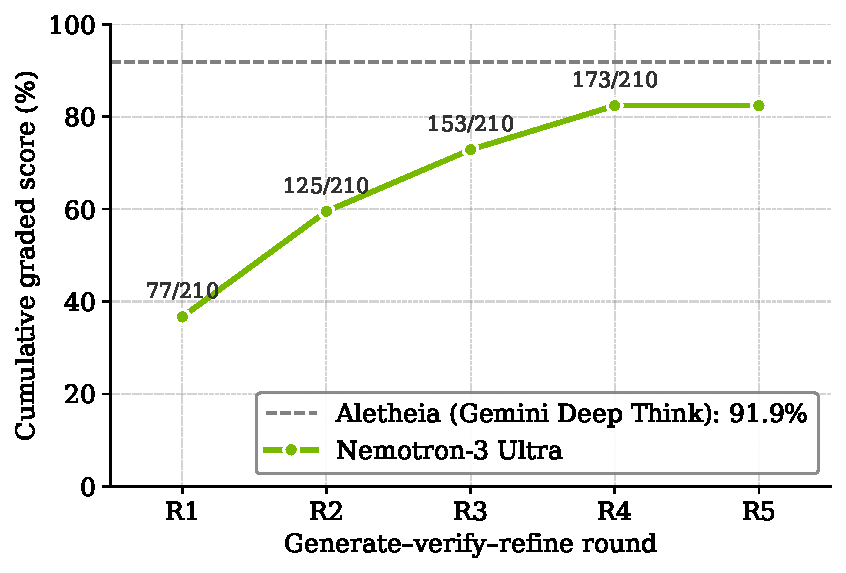
\includegraphics[width=\linewidth]{figures/math_ttc.pdf}
\captionof{figure}{Test-time scaling of \ourmodel on IMO-ProofBench Advanced by round}
\label{fig:math_ttc}
\end{minipage}
\end{figure*}

\subsubsection{Test-time Scaling in Math Olympiad Problems}

\ourmodel achieves strong performance as the underlying model of a high-compute, search-based test-time scaling strategy for Olympiad-level competition mathematics. Following the generate--verify--refine methodology of \citet{shao2025deepseekmath}\footnote{In contrast with the original paper, we started with 128 proof attempts per problem and allowed 512k context length. All other pipeline hyperparameters were identical.} and Nemotron-Cascade-2~\citep{yang2026nemotron}, we evaluate on the IMO-ProofBench Advanced subset \citep{luong2025towards}, IMO 2025, Putnam 2025, and USAMO 2026, with final accuracies reported in Table~\ref{tab:math_ttc}.

Figure~\ref{fig:math_ttc} shows the accuracy of the test-time scaling strategy vs rounds of refinement in the pipeline, as a proxy for compute. The SOTA performance of the Aletheia math research agent \citep{feng2026autonomousmathematicsresearch} is also plotted.




% \subsection{SFT}
% \subsection{MOPD}
% \subsubsection{Ultra Agentic Teacher training}
% \subsubsection{Ultra Reasoning Teacher training}
% \subsection{RL based post-training}
% \subsection{RLHF}
% \subsubsection{Reward modeling}


